% !TEX root = FDS_Technical_Reference_Guide.tex

\typeout{new file: Appendices.tex}

\chapter{Nomenclature}
\label{nomenclature}

\begin{tabbing}
$A_{\rm p,c}$ \hspace{1in}\= droplet/particle cross sectional area \\
$A_{\rm p,s}$ \hspace{1in}\= droplet/particle surface area \\
$A_{\alpha\beta}$         \> pre-exponential factor for solid phase Arrhenius reaction \\
B                       \> emission source term; particle mobility \\
$C$                       \> sprinkler C-factor; coefficient of natural convection \\
$C_{\rm d}$               \> drag coefficient \\
$C_{\rm m}$               \> momentum accommodation coefficient \\
Cn                        \> Cunningham slip correction factor \\
$C_{\rm s}$               \> Smagorinsky constant (LES); thermal slip coefficient  \\
$C_{\rm t}$               \> thermal accommodation coefficient \\
$c$                       \> solid material specific heat; speed of light in vacuum \\
$c_p$                     \> constant-pressure specific heat \\
$D$                       \> droplet/particle diameter   \\
$D_{\alpha}$              \> diffusion coefficient \\
$D_{\rm v,0.5}$           \> median volumetric droplet diameter \\
$E$                       \> activation energy \\
Fu                        \> Fuchs factor \\
$\bof_{\rm b}$            \> external force vector (excluding gravity) \\
$g$                       \> acceleration of gravity \\
$\bg$                     \> gravity vector, normally $(0,0,-g)$ \\
$\cH$                      \> total pressure divided by the density (Bernoulli integral)\\
$H_{{\rm r},\alpha\beta}$ \> heat of reaction for a solid phase reaction     \\
$h$                       \> heat transfer coefficient; Planck constant      \\
$h_{\rm s,\alpha}$        \> sensible enthalpy of species $\alpha$   \\
$I$                       \> radiation intensity per unit of solid angle     \\
$I_{\rm b}$               \> radiation blackbody intensity per unit of solid angle  \\
$I_{b,\rm \la}$           \> spectral radiation blackbody intensity as function of wavelength per unit of solid angle  \\
$I_{b,\rm \om}$           \> spectral radiation blackbody intensity as function of wavenumber per unit of solid angle  \\
$k$                       \> thermal conductivity; suppression decay factor \\
$k_{\rm B}$               \> Boltzmann constant                             \\
Kn                        \> Knudsen number \\
$K_{\rm th}$              \> thermophoretic velocity coefficient \\
$L$                       \> characteristic length; surface thickness \\
$\dm_{{\rm b},\alpha}'''$ \> mass production rate per unit volume of species $\alpha$ by evaporating droplets/particles \\
$\dm_\alpha'''$           \> mass production rate per unit volume of species $\alpha$ by chemical reactions \\
$\dm_{\rm w}''$           \> water mass flux  \\
$m_{\rm w}''$             \> water mass per unit area \\
$n_{\rm s}$               \> partial reaction order for solid \\
$n_{\rm O_2}$             \> partial reaction order for oxygen \\
$\NU$                     \> Nusselt number \\
$\PR$                     \> Prandtl number \\
$p$                       \> pressure \\
$\bp_0$                   \> atmospheric pressure profile \\
$\bp_m$                   \> background pressure of $m$th pressure zone \\
$\tp$                     \> pressure perturbation \\
$\dbq''$                  \> heat flux vector \\
$\dq'''$                  \> heat release rate per unit volume \\
$\dq_{\rm r}''$           \> radiative heat flux \\
$\dq_{\rm c}''$           \> convective heat flux \\
$\dQ$                     \> total heat release rate \\
$\dQ^*$                   \> fire Froude number \\
$\R$                      \> universal gas constant \\
Re                        \> Reynolds number \\
$r_{\rm p}$               \> particle/droplet radius \\
$r_{\alpha\beta}$         \> solid phase reaction rate \\
RTI                       \> Response Time Index of a sprinkler \\
$\bs$                     \> unit vector in direction of radiation intensity \\
$\SC$                     \> Schmidt number \\
$\SH$                     \> Sherwood number \\
$S_\alpha$                \> solid component production rate \\
$T$                       \> temperature \\
$t$                       \> time           \\
$U$                       \> integrated radiant intensity; optical pathlength \\
$\bu=(u,v,w)$             \> velocity vector  \\
$W_\alpha$                \> molecular weight of gas species $\alpha$ \\
$\bW$                     \> molecular weight of the gas mixture \\
$\WE$                     \> Weber number \\
$\bx=(x,y,z)$             \> position vector  \\
$X_\alpha$                \> volume fraction of species $\alpha$   \\
$Y_\alpha$                \> mass fraction of species $\alpha$   \\
$\bar{Y}_\alpha$          \> mean mass fraction of species $\alpha$   \\
$\hat{Y}_\alpha$          \> mass fraction of species $\alpha$ in mixed zone of a computation cell \\
$Y_\OTWO^\infty$          \> mass fraction of oxygen in the ambient   \\
$Y_{\rm F}$               \> mass fraction of fuel   \\
$y_{\rm s}$               \> soot yield \\
$Z_\alpha$                \> species mixture $\alpha$   \\
\hspace{0.1in}            \> \\
{\bf Greek Letters}       \> \\
\hspace{0.1in}            \> \\
$\alpha$                  \> ratio of gas conductivity to the particle conductivity; integrated band intensity \\
$\gamma$                  \> ratio of specific heats; Rosin-Rammler exponent; spectral fine structure parameter of narrow band \\
$\Delta$                  \> LES filter width \\
$\Delta h$                \> heat of combustion \\
$\Delta h_\OTWO$          \> energy released per unit mass oxygen consumed \\
$\Delta h_{\rm f,\alpha}^0$ \> heat of formation of species $\alpha$ \\
$\delta$                  \> film thickness; scaling factor of thickness and density \\
$\epsilon$                \> dissipation rate; emissivity; agglomeration factor \\
$\eta$                    \> agglomeration apportioning factor \\
$\kappa$                  \> absorption coefficient; von Karman constant \\
$\lambda$                 \> mean free path of gas molecules; wavelength of thermal radiation\\
$\mu$                     \> dynamic viscosity \\
$\nu$                     \> frequency of the thermal radiation \\
$\nu_\alpha$              \> stoichiometric coefficient, species $\alpha$ \\
$\nu_{\rm s}$             \> yield of solid residue in solid phase reaction \\
$\nu_{{\rm g},\gamma}$    \> yield of gaseous species $\gamma$ in solid phase reaction \\
$\rho$                    \> density \\
$\bar{\tau}_{\om}$        \> mean spectral transmissivity of a narrow band centered in $\om$ \\
$\btau_{ij}$              \> viscous stress tensor \\
$\Phi$                    \> agglomeration kernel \\
$\phi$                    \> porosity \\
$\chi$                    \> shape factor \\
$\chi_{\rm r}$            \> radiative loss fraction \\
$\sigma$                  \> Stefan-Boltzmann constant; constant in droplet size distribution; surface tension \\
$\sigma_{\rm p}$          \> particle scattering coefficient \\
$\sigma_{\rm s}$          \> scattering coefficient \\
$\tau^+$                  \> dimensionless stopping distance \\
$\om$                     \> wavenumber of thermal radiation \\
$\bo=(\omx,\omy,\omz)$    \> vorticity vector \\
$\Omega$                  \> solid angle \\
\hspace{0.1in}            \> \\
{\bf Subscripts}          \> \\
\hspace{0.1in}            \> \\
0                         \> initial value \\
a                         \> air \\
b                         \> bulk phase property; boiling \\
B                         \> Brownian \\
c                         \> convective \\
d                         \> drag \\
e                         \> effective properties \\
g                         \> gas \\
$ijk$                     \> gas phase cell indices \\
n                         \> band properties \\
p                         \> particle/droplet \\
PK                        \> collision efficiency \\
$p$                       \> pressure \\
r                         \> radiative \\
s                         \> solid; sensible; soot\\
S                         \> sticking factor \\
w                         \> wall \\
$\alpha$                  \> gas species index \\
$\beta$                   \> index of reaction \\
$\la$                     \> wavelength \\
$\om$                     \> wavenumber \\
\end{tabbing}





\chapter{A Velocity Divergence Constraint for Large-Eddy Simulation of Low-Mach Flows}
\label{app_divergence}

The equations governing the evolution of a low-Mach, variable density fluid---first introduced by Rehm and Baum in 1978 \cite{Rehm:1}---are continuity, species concentration (mass fraction), momentum, energy (sensible enthalpy), and the ideal gas equation of state:
\begin{gather}
\label{eqn_rho} \frac{\partial \rho}{\partial t} + \Div(\rho\mathbf{u}) = \dot{m}_{\rm b}''' \\
\label{eqn_Y_a} \frac{\partial \rho Y_\alpha}{\partial t} + \Div(\rho Y_\alpha \mathbf{u}) = \Div (\rho D_\alpha \nabla Y_\alpha) + \dot{m}_\alpha^\tripleprime + \dot{m}_{{\rm b},\alpha}^\tripleprime \\
\label{eqn_u}   \frac{\partial \rho \mathbf{u}}{\partial t} + \Div(\rho \mathbf{u} \mathbf{u}) = -\nabla \tilde{p} - \Div\mathbf{\tau} + (\rho-\rho_0) \mathbf{g} \\
\label{eqn_h_s} \frac{\partial \rho h_s}{\partial t} + \Div(\rho h_s \mathbf{u}) = \frac{\mbox{D} \bar{p}}{\mbox{D} t} + \dot{q}^\tripleprime - \Div \dot{\mathbf{q}}^\pp \\
\label{eqn_eos} \rho = \frac{\bar{p} \overline{W}}{RT}
\end{gather}
In this appendix, starting from the conservative form of the sensible enthalpy transport equation, we derive a numerically consistent velocity divergence constraint for use in large-eddy simulation (LES) of low-Mach flows.  The result accounts for numerical transport of mass and energy, which is difficult to eliminate in relatively coarse, engineering LES calculations when total variation diminishing (TVD) scalar transport schemes are employed.  Without the correction terms derived here, unresolved (numerical) mixing of gas species with different heat capacities and molecular weights may lead to erroneous mixture temperatures and ultimately to an imbalance in the energy budget.

\section{The Divergence Constraint}
\label{div_constraint}

As mentioned, the present work stems from attempts to understand and correct an energy budget imbalance that became evident after implementing both temperature-dependent specific heats and TVD scalar transport. One of the revelations of this work has been that the choice of starting point for deriving the divergence constraint naturally leads to two different forms of the divergence expression.  While these forms are mathematically equivalent, they lead to two completely different---and yet completely plausible---numerical formulations.

\subsection{From Continuity}
Starting from the continuity equation, we can factor out the velocity divergence leaving the material derivative of the density:
\begin{align}
\Div\mathbf{u} &= -\frac{1}{\rho}\frac{\D\rho}{\D t} + \frac{1}{\rho} \dot{m}_{\rm b}'''
\end{align}
Using the ideal gas law and differentiating the equation of state leads to
\begin{align}
\label{eqn_div_1}
\Div\mathbf{u} &= \left(\frac{1}{\rho c_p T} - \frac{1}{\bar{p}} \right)\frac{\mbox{D} \bar{p}}{\mbox{D} t} \notag\\[.1in]
&+ \frac{1}{\rho c_p T} \left[ \dot{q}^\tripleprime - \Div \dot{\mathbf{q}}^\pp \right] \notag\\[.1in]
&+ \frac{1}{\rho} \sum_\alpha \left(\frac{\overline{W}}{W_\alpha} - \frac{h_{s,\alpha}}{c_p T} \right) \big[ \Div (\rho D_\alpha \nabla Y_\alpha) + \dot{m}_\alpha^\tripleprime \big] \notag \\[.1in]
&+ \frac{1}{\rho} \sum_\alpha \left(\frac{\overline{W}}{W_\alpha} - \frac{\int_{T_{\rm b}}^T c_{p,\alpha}(T') \, {\rm d}T'}{c_p T} \right) \, \dot{m}_{\rm b,\alpha}^\tripleprime
\end{align}

\subsection{From Sensible Enthalpy}
Alternatively, we may factor the velocity divergence from the sensible enthalpy transport equation:
\begin{align}
\label{eqn_div_new}
\Div\mathbf{u} &= \frac{1}{\rho h_s} \left[ \frac{\D}{\D t}(\bar{p}-\rho h_s) + \dot{q}^\tripleprime - \Div \dot{\mathbf{q}}^\pp \right]
\end{align}
From this starting point, (arguably) the natural result for the divergence expression is
\begin{align}
\label{eqn_div_2}
\Div\mathbf{u} &= \frac{1}{\rho c_p T}\frac{\mbox{D} \bar{p}}{\mbox{D} t} - \frac{1}{\bar{p}} \frac{\partial \bar{p}}{\partial t} \notag\\[.1in]
&+ \frac{1}{\rho c_p T}\left[ \dot{q}^\tripleprime - \Div \dot{\mathbf{q}}^\pp - \mathbf{u} \cdot\nabla (\rho h_s) \right] \notag\\[.1in]
&+ \frac{1}{\rho} \sum_\alpha \left(\frac{\overline{W}}{W_\alpha} - \frac{h_{s,\alpha}}{c_p T} \right) \big[ \Div (\rho D_\alpha \nabla Y_\alpha) - \mathbf{u} \cdot \nabla (\rho Y_\alpha) + \dot{m}_\alpha^\tripleprime \big] \notag \\[.1in]
&+ \frac{1}{\rho} \sum_\alpha \left(\frac{\overline{W}}{W_\alpha} - \frac{\int_{T_{\rm b}}^T c_{p,\alpha}(T') \, {\rm d}T'}{c_p T} \right) \, \dot{m}_{\rm b,\alpha}^\tripleprime
\end{align}

\subsection{Comparison}
Notice the subtle differences between the first, second, and third lines of (\ref{eqn_div_1}) and (\ref{eqn_div_2}).  The first lines differ by $\displaystyle (\mathbf{u}\cdot\nabla \bar{p})/\bar{p}$. In (\ref{eqn_div_2}), the second and third lines each contain an extra term accounting for advection of enthalpy and mass, respectively, $\mathbf{u} \cdot\nabla (\rho h_s)$ and $\mathbf{u} \cdot \nabla (\rho Y_\alpha)$.  Using (\ref{eqn_rho})-(\ref{eqn_eos}), it can be shown that (\ref{eqn_div_1}) and (\ref{eqn_div_2}) are mathematically equivalent (see Section \ref{app_div_equivalence}).


\section{The Discrete Divergence}
\label{discrete_divergence}

The \emph{conservative form} of the sensible enthalpy transport equation---which derives its name from the flux divergence form of the mean transport term on the left hand side---is
\begin{equation}
\label{eqn_conservative_enthalpy}
\frac{\partial (\rho h_s)}{\partial t} + \underbrace{\Div(\rho h_s \mathbf{u})}_{\mbox{mean transport}} = \frac{\D \bar{p}}{\D t} + \dot{q}^\tripleprime - \Div \dot{\mathbf{q}}^\pp \,\mbox{.}
\end{equation}
This form is called conservative because, by Gauss's theorem, the integral of the discrete flux divergence over the domain is equivalent to the surface integral of the flux over the boundary of the domain.  For a periodic domain the integral is zero---\emph{flow in} must equal \emph{flow out}. The key to guaranteeing discrete conservation of sensible enthalpy is to first discretize the mean transport term.  Below an overline will denote a slope-limiting interpolation operator.  As discussed in Section \ref{app_transport_decomposition}, this operator is specially designed to be consistent with flux-limited, total variation diminishing (TVD) transport for the conservative form of the mean transport term.

Expanding the mean transport term and rearranging (\ref{eqn_conservative_enthalpy}) in terms of the discrete divergence yields
\begin{equation}
\label{eqn_discrete_divergence}
\Div \mathbf{u} = \frac{1}{\rho h_s}\left[ -\left( \frac{\partial (\rho h_s)}{\partial t} + \overline{\mathbf{u}\cdot\nabla(\rho h_s)} \right) + \frac{\D \bar{p}}{\D t} + \dot{q}^\tripleprime - \Div \dot{\mathbf{q}}^\pp \right] \,\mbox{.}
\end{equation}
The numerical details of $\overline{\mathbf{u}\cdot\nabla(\rho h_s)}$ are the key to assuring discrete conservation (see Section \ref{app_transport_decomposition}). Mathematically, (\ref{eqn_discrete_divergence}) is  equivalent to (\ref{eqn_div_new}). Numerically, however, (\ref{eqn_discrete_divergence}) accounts for the critical details of the TVD transport scheme.

Most of the complexity in the divergence expression is buried in the time derivative term, $\partial (\rho h_s)/\partial t$.  Using (\ref{eqn_rho})-(\ref{eqn_eos}), it can be shown that (\ref{eqn_discrete_divergence}) expands to yield (\ref{eqn_div_2}) (see Section \ref{app_time_derivative}).


\subsection{Factoring the Discrete Flux Divergence}
\label{app_transport_decomposition}

Below we show the numerical decomposition of the enthalpy flux divergence for cell $i$ in 1D.  The operator $\delta(\,\,\,)/\delta x$ denotes a central difference.  Density $\rho$ and sensible enthalpy $h_s$ are stored at cell centers indexed by $i$, $i+1$, etc.  Velocity $u$ is stored at the cell face and indexed by $i+\mhalf$, etc.  Here an overline applied to a face value ($i\pm\mhalf$ suffix) denotes a flux limiter, which is basically a special interpolation of the scalar field to the cell face.  The purpose of the flux limiter is to prevent spurious oscillations in the scalar solution.  Such oscillations must be avoided because they may lead to boundedness violations and instability.

In decomposing the flux divergence, our goal is to break the term into two parts as follows:
\begin{align}
\label{eqn_flux_decomposition}
\left[\frac{\delta (\rho h_s u)}{\delta x}\right]_i &= \frac{ \overline{(\rho h_s)}_{i+\thalf} u_{i+\thalf} - \overline{(\rho h_s)}_{i-\thalf} u_{i-\thalf} }{\delta x} \notag\\
&= (\rho h_s)_i \underbrace{\frac{u_{i+\thalf}-u_{i-\thalf}}{\delta x}}_{\displaystyle\Div\mathbf{u}} + \underbrace{\frac{\Delta_{i+\thalf} u_{i+\thalf} + \Delta_{i-\thalf} u_{i-\thalf}}{\delta x}}_{\displaystyle\overline{\mathbf{u}\cdot\nabla(\rho h_s)}}
\end{align}
Here $\Delta_{i+\thalf}$ represents a limited slope of the scalar data ($\rho h_s$ in this case) at the face $i+\frac{1}{2}$.  The slope limiters for cell $i$ are defined such that
\begin{align}
\label{eqn_slope_1} (\rho h_s)_i + \Delta_{i+\thalf} = \overline{(\rho h_s)}_{i+\thalf} \\
\label{eqn_slope_2} (\rho h_s)_i - \Delta_{i-\thalf} = \overline{(\rho h_s)}_{i-\thalf}
\end{align}

Note that while scalar face values are unique to the face $\left[\overline{(\rho h_s)}_{i+\thalf} = \overline{(\rho h_s)}_{i+1-\thalf}\right]$, the limited slopes are not ($\Delta_{i+\thalf} \ne \Delta_{i+1-\thalf}$).

\subsection{Example: Pure Upwinding}
Suppose all $u>0$ in 1D, a wind from left to right.  For Godunov's scheme (first-order upwinding) the limited slopes would be computed as follows:
\begin{align}
\Delta_{i+\thalf} &= \overline{(\rho h_s)}_{i+\thalf} - (\rho h_s)_i \notag\\
&= (\rho h_s)_i - (\rho h_s)_i \notag\\
&= 0
\end{align}
\begin{align}
\Delta_{i-\thalf} &= (\rho h_s)_i - \overline{(\rho h_s)}_{i-\thalf} \notag\\
&= (\rho h_s)_i - (\rho h_s)_{i-1}
\end{align}
The cell-average advection term therefore becomes
\begin{align}
\overline{\mathbf{u}\cdot\nabla(\rho h_s)} &= u_{i-\thalf} \left[ \frac{(\rho h_s)_i - (\rho h_s)_{i-1}}{\delta x} \right]
\end{align}

\subsection{Example: Central Differencing}
For central differencing the limited slopes would be computed as follows:
\begin{align}
\Delta_{i+\thalf} &= \overline{(\rho h_s)}_{i+\thalf} - (\rho h_s)_i \notag\\
&= \frac{1}{2}\left[(\rho h_s)_i + (\rho h_s)_{i+1}\right] - (\rho h_s)_i \notag\\
&= \frac{1}{2}\left[(\rho h_s)_{i+1} - (\rho h_s)_i\right]
\end{align}
\begin{align}
\Delta_{i-\thalf} &= (\rho h_s)_i - \overline{(\rho h_s)}_{i-\thalf} \notag\\
&= (\rho h_s)_i - \frac{1}{2}\left[(\rho h_s)_{i-1} + (\rho h_s)_i\right] \notag\\
&= \frac{1}{2}\left[ (\rho h_s)_i - (\rho h_s)_{i-1} \right]
\end{align}
The cell-average advection term therefore becomes
\begin{align}
\overline{\mathbf{u}\cdot\nabla(\rho h_s)} &= \frac{1}{2}  u_{i+\thalf} \left[ \frac{(\rho h_s)_{i+1} - (\rho h_s)_i}{\delta x} \right] + \frac{1}{2} u_{i-\thalf} \left[ \frac{(\rho h_s)_i - (\rho h_s)_{i-1}}{\delta x} \right]
\end{align}

\subsection{General Implementation: Using Flux Limiters}
The examples above are for illustration purposes only.  In general, we first compute the flux-limited face values and obtain the limited slopes from (\ref{eqn_slope_1}) and (\ref{eqn_slope_2}).  The cell-average advection term is then computed from the second underbrace in (\ref{eqn_flux_decomposition}).


\section{Decomposing the Time Derivative}
\label{app_time_derivative}

Using the ideal gas law, the time derivative of the enthalpy can be decomposed as follows:
\begin{align}
\label{eqn_drhdt}
\frac{\partial (\rho h_s)}{\partial t} &= \rho \frac{\partial h_s}{\partial t} + h_s \frac{\partial \rho}{\partial t} \notag\\
&= \rho \sum_\alpha \left( Y_\alpha c_{p,\alpha} \frac{\partial T}{\partial t} + h_{s,\alpha} \frac{\partial Y_\alpha}{\partial t}\right) + h_s \frac{\partial \rho}{\partial t} \notag\\
&= \rho c_p \frac{\partial T}{\partial t} + \rho \sum_\alpha h_{s,\alpha} \frac{\partial Y_\alpha}{\partial t} + h_s \frac{\partial \rho}{\partial t} \notag\\
&= \rho c_p T \left[ \frac{1}{\bar{p}} \frac{\partial \bar{p}}{\partial t} + \frac{1}{\overline{W}} \frac{\partial \overline{W}}{\partial t} - \frac{1}{\rho} \frac{\partial \rho}{\partial t}\right] + \rho \sum_\alpha h_{s,\alpha} \frac{\partial Y_\alpha}{\partial t} + h_s \frac{\partial \rho}{\partial t} \notag\\
&= \rho c_p T \left[ \frac{1}{\bar{p}} \frac{\partial \bar{p}}{\partial t} - \sum_\alpha \frac{\overline{W}}{W_\alpha} \frac{\partial Y_\alpha}{\partial t} - \frac{1}{\rho} \frac{\partial \rho}{\partial t}\right] + \rho \sum_\alpha h_{s,\alpha} \frac{\partial Y_\alpha}{\partial t} + h_s \frac{\partial \rho}{\partial t} \notag\\
&=  \frac{\rho c_p T}{\bar{p}} \frac{\partial \bar{p}}{\partial t}  + \rho \sum_\alpha \left( h_{s,\alpha} - c_p T \frac{\overline{W}}{W_\alpha}\right)\frac{\partial Y_\alpha}{\partial t} + (h_s - c_p T) \frac{\partial \rho}{\partial t}
\end{align}
The time derivative of the mass fractions, which originates from the species transport equation, is:
\begin{align}
\label{eqn_dydt}
\frac{\partial Y_\alpha}{\partial t} &= \frac{1}{\rho} \left[ \Div (\rho D_\alpha \nabla Y_\alpha) + \dot{m}_\alpha^\tripleprime - Y_\alpha \frac{\partial \rho}{\partial t} - \Div (\rho Y_\alpha \mathbf{u}) \right]
\end{align}
Using (\ref{eqn_dydt}) in (\ref{eqn_drhdt}) and summing over species to eliminate the density time derivative we obtain
\begin{align}
\label{eqn_drhdt2}
\frac{\partial (\rho h_s)}{\partial t} &= \frac{\rho c_p T}{\bar{p}} \frac{\partial \bar{p}}{\partial t}  + \sum_\alpha \left( h_{s,\alpha} - c_p T \frac{\overline{W}}{W_\alpha}\right)\left[ \Div (\rho D_\alpha \nabla Y_\alpha) + \dot{m}_\alpha^\tripleprime - \mathbf{u}\cdot\nabla(\rho Y_\alpha) - \rho Y_\alpha \Div \mathbf{u} \right]
\end{align}
Plugging (\ref{eqn_drhdt2}) into (\ref{eqn_div_new}) yields (almost done)
\begin{align}
\label{eqn_div_3}
\Div \mathbf{u} &= \frac{1}{\rho h_s}\frac{\mbox{D} \bar{p}}{\mbox{D} t} - \frac{c_p T}{h_s}\frac{1}{\bar{p}} \frac{\partial \bar{p}}{\partial t} \notag\\
&+ \frac{1}{\rho h_s}\left[ \dot{q}^\tripleprime - \Div \dot{\mathbf{q}}^\pp - \mathbf{u} \cdot\nabla (\rho h_s) \right] \notag\\
&+ \frac{1}{\rho h_s} \sum_\alpha \left(c_p T\frac{\overline{W}}{W_\alpha} - h_{s,\alpha} \right) \bigg[ \Div (\rho D_\alpha \nabla Y_\alpha) - \mathbf{u} \cdot \nabla (\rho Y_\alpha) - \rho Y_\alpha \Div \mathbf{u} \bigg] \notag\\
&+ \frac{1}{\rho h_s} \sum_\alpha \left(c_p T\frac{\overline{W}}{W_\alpha} - h_{s,\alpha} \right) \dot{m}_\alpha^\tripleprime
\end{align}
\begin{align}
\label{eqn_div_4}
\Div \mathbf{u} + \frac{1}{\rho h_s} \sum_\alpha \left(c_p T\frac{\overline{W}}{W_\alpha} - h_{s,\alpha} \right) \rho Y_\alpha \Div \mathbf{u}  &= \frac{1}{\rho h_s}\frac{\mbox{D} \bar{p}}{\mbox{D} t} - \frac{c_p T}{h_s}\frac{1}{\bar{p}} \frac{\partial \bar{p}}{\partial t} \notag\\
&+ \frac{1}{\rho h_s}\left[ \dot{q}^\tripleprime - \Div \dot{\mathbf{q}}^\pp - \mathbf{u} \cdot\nabla (\rho h_s) \right] \notag\\
&+ \frac{1}{\rho h_s} \sum_\alpha \left(c_p T\frac{\overline{W}}{W_\alpha} - h_{s,\alpha} \right) \bigg[ \Div (\rho D_\alpha \nabla Y_\alpha) - \mathbf{u} \cdot \nabla (\rho Y_\alpha) + \dot{m}_\alpha^\tripleprime\bigg]
\end{align}
\begin{align}
\label{eqn_div_5}
\Div \mathbf{u} + \left(\frac{c_p T}{h_s} - 1\right)\Div \mathbf{u}  &= \frac{1}{\rho h_s}\frac{\mbox{D} \bar{p}}{\mbox{D} t} - \frac{c_p T}{h_s}\frac{1}{\bar{p}} \frac{\partial \bar{p}}{\partial t} \notag\\
&+ \frac{1}{\rho h_s}\left[ \dot{q}^\tripleprime - \Div \dot{\mathbf{q}}^\pp - \mathbf{u} \cdot\nabla (\rho h_s) \right] \notag\\
&+ \frac{1}{\rho h_s} \sum_\alpha \left(c_p T\frac{\overline{W}}{W_\alpha} - h_{s,\alpha} \right) \bigg[ \Div (\rho D_\alpha \nabla Y_\alpha) - \mathbf{u} \cdot \nabla (\rho Y_\alpha) + \dot{m}_\alpha^\tripleprime \bigg]
\end{align}
Finally... (compare with (\ref{eqn_div_2}))
\begin{align}
\label{eqn_div_6}
\Div \mathbf{u} &= \frac{1}{\rho c_p T}\frac{\mbox{D} \bar{p}}{\mbox{D} t} - \frac{1}{\bar{p}} \frac{\partial \bar{p}}{\partial t} \notag\\
&+ \frac{1}{\rho c_p T}\left[ \dot{q}^\tripleprime - \Div \dot{\mathbf{q}}^\pp - \mathbf{u} \cdot\nabla (\rho h_s) \right] \notag\\
&+ \frac{1}{\rho} \sum_\alpha \left(\frac{\overline{W}}{W_\alpha} - \frac{h_{s,\alpha}}{c_p T} \right) \bigg[ \Div (\rho D_\alpha \nabla Y_\alpha) - \mathbf{u} \cdot \nabla (\rho Y_\alpha) + \dot{m}_\alpha^\tripleprime \bigg]
\end{align}

\section{Equivalence between Divergence Expressions}
\label{app_div_equivalence}

The equivalence between (\ref{eqn_div_1}) and (\ref{eqn_div_2}) is apparent based on the following:
\begin{flalign}
-\frac{1}{\rho c_p T} \mathbf{u}\cdot\nabla(\rho h_s) - \frac{1}{\rho} \sum_\alpha \left( \frac{\overline{W}}{W_\alpha} - \frac{h_{s,\alpha}}{c_p T} \right) \mathbf{u}\cdot\nabla(\rho Y_\alpha) &&\notag
\end{flalign}
\vskip-\baselineskip
\begin{align}
&= -\frac{1}{\rho c_p T} \left[ \rho \mathbf{u}\cdot\nabla h_s + h_s \mathbf{u}\cdot\nabla \rho \right] - \frac{1}{\rho} \sum_\alpha \left( \frac{\overline{W}}{W_\alpha} - \frac{h_{s,\alpha}}{c_p T} \right) \left[ \rho \mathbf{u}\cdot\nabla Y_\alpha + Y_\alpha \mathbf{u}\cdot\nabla \rho \right] \notag\\
&= -\frac{1}{c_p T} \mathbf{u}\cdot \sum_\alpha \left[ Y_\alpha \nabla h_{s,\alpha} + h_{s,\alpha} \nabla Y_\alpha \right] - \frac{1}{\rho} \mathbf{u}\cdot\nabla \rho - \sum_\alpha \left( \frac{\overline{W}}{W_\alpha} - \frac{h_{s,\alpha}}{c_p T} \right) \mathbf{u}\cdot\nabla Y_\alpha \notag\\
&= -\frac{1}{c_p T} \mathbf{u}\cdot \sum_\alpha Y_\alpha \nabla h_{s,\alpha} - \frac{1}{\rho} \mathbf{u}\cdot\nabla \rho - \sum_\alpha \frac{\overline{W}}{W_\alpha} \mathbf{u}\cdot\nabla Y_\alpha \notag\\
&= -\frac{1}{c_p T} \mathbf{u}\cdot \sum_\alpha Y_\alpha c_{p,\alpha} \nabla T - \frac{1}{\rho} \mathbf{u}\cdot\nabla \rho - \mathbf{u}\cdot \sum_\alpha \overline{W} \nabla (Y_\alpha/W_\alpha) \notag\\
&= -\mathbf{u}\cdot \left[\frac{1}{T} \nabla T + \frac{1}{\rho} \nabla \rho + \overline{W} \nabla (1/\overline{W}) \right] \notag\\
&= -\frac{1}{\bar{p}} \mathbf{u}\cdot \nabla \bar{p}
\end{align}


\section{Simplifications for Constant Specific Heat}

Recall that for an ideal gas we may write
\begin{align}
c_{p,\alpha} = c_{v,\alpha} + R/W_\alpha = \frac{R}{W_\alpha} \left(\frac{\gamma_\alpha}{\gamma_\alpha-1}\right) \,\mbox{,}
\end{align}
where $c_{p,\alpha}$ is the specific heat of $\alpha$ at constant pressure, $c_{v,\alpha}$ is the specific heat at constant volume, and $\gamma_\alpha = c_{p,\alpha}/c_{v,\alpha}$.  Commonly, the ratio of specific heats is approximated to be constant, and for fire calculations typically the value for air is chosen, $\gamma \approx 1.4$.  If we take the reference temperature to be zero, the sensible enthalpy in this case becomes
\begin{align}
\rho h_s = \rho c_p T = \rho T \sum_\alpha Y_\alpha c_{p,\alpha} = \rho R T \left(\frac{\gamma}{\gamma-1}\right)\sum_\alpha \frac{Y_\alpha}{W_\alpha} = \rho \frac{R T}{\overline{W}} \left(\frac{\gamma}{\gamma-1}\right) = \bar{p}\left(\frac{\gamma}{\gamma-1}\right)
\end{align}
Therefore, if $\bar{p}$ is constant and uniform then $\rho h_s$ is constant and uniform.  Consequently, $\partial (\rho h_s)/\partial t = 0$ and $\nabla (\rho h_s) = 0$, so we require no corrections to the divergence expression.  This improves the speed of the code since these divergence corrections are rather expensive.  To employ this simplification, the user enters \emph{both} {\ct CONSTANT\_SPECIFIC\_HEAT\_RATIO=.TRUE.} and {\ct STRATIFICATION=.FALSE.} on the {\ct MISC} line of the input file.


%\chapter{Multi-environment Extension of Reactor Model}
%
%\label{multi_env_edc}
%
%In the current formulation of the reactor model FDS does not transport the mixing variable. At the start of a time step, mixing is assumed to be in the unmixed state. We would like to extend the reactor model so that we can eventually construct PDFs of reactor concentration. The difficulty is how to construct/transport the necessary information to build the PDF.
%
%One efficient way to describe a PDF is to use moments; where a moment can be thought of a statistical descriptor of the distribution. The first moment of a distribution is the mean of the distribution, the second is the variance, etc. Therefore, the more moments we know, the better the description of the distribution we have. For a given PDF, p(y), the $k^{th}$ moment of $y$ of the distribution is:
%\begin{equation}\label{eq:int_moment}
%_{y}M_{k} = \int y^{k}p(y)\mathrm{d}y
%\end{equation}
%Solving this integral equation can become difficult as it requires the function form of the PDF. An alternative way to compute moments is to use Gaussian-quadrature, which represents the moment integral in Eq.~\ref{eq:int_moment} as an n-point sum \cite{mcgraw:1997}:
%\begin{equation}\label{eq:qmom}
%_{y}M_{k}=\displaystyle \sum_{i=1}^{n} \hat y_{i}^{k} w_{i}
%\end{equation}
%This technique is known as the quadrature method of moments (QMOM) where  $\hat y_i^k$ is known at the $i^{th}$ quadrature point, $w_i$ is known as the $i^{th}$ quadrature weight, and $n$ is the number of quadrature points. If we consider the unmixed fraction as a weight describing the amount of mixing, the steps to obtain higher order statistics about the batch reactor composition begin to take shape. The unmixed fraction, $\zeta$, exists in two probabilistic states: $p1$ and $p2$, where $p2 = 1-p1$. State 1 ($p1$) describes the amount of the cell that is mixed while state 2 ($p2$) describes the unmixed portion. If we know the mass fractions of species in both mixing states (quadrature points) and the corresponding weights to those states, then we can use QMOM to construct the reactor distribution.
%
%In this case, the quadrature weights become the unmixed fraction, $\zeta_{i}$, and the quadrature points become the mass fractions $\phi_{\alpha,i}$. Applying Eq.~\ref{eq:qmom}, the moments of the distribution in the reactor are:
%\begin{eqnarray}\label{eq:moments}
%M_{0} &=& \displaystyle \sum_{i=1}^{n} \zeta_{i} \\
%\nonumber M_{1} &=& \displaystyle \sum_{i=1}^{n} \zeta_{i} \phi_{\alpha,i} \\
%\nonumber M_{2} &=& \displaystyle \sum_{i=1}^{n} \zeta_{i} \phi_{\alpha,i}^2
%\end{eqnarray}
%The mean of the distribution becomes $M_{1}$ and the centered variance becomes $M_{2}-M_{1}^{2}$. To implement subgrid statistics in FDS, we would either need to transport the unmixed fraction or develop a model for the subgrid variance. Since scalar transport is expensive, a first approach is to develop a model to approximate the subgrid variance. If the variance is known, QMOM can then be used to solve for the initial unmixed fraction.


\chapter{Absorption Coefficients of Gaseous Fuels}
\label{absorption_coefficients}

For the calculation of the gray or band-mean absorption coefficients, $\kappa_n$, a narrow-band model, RADCAL~\cite{RadCal}, has been
implemented in FDS. RADCAL computes the spectral properties of the radiation participating species at discrete values of the spectrum (expressed either in wavenumber $\om$ or in wavelength $\la$) and temperature,
and returns two alternative mean absorption coefficients for each spectral band, $n$. The first coefficient is the Planck mean coefficient \cite{Tien:1968}
\begin{equation}
\kappa_n(P,T) = \dfrac{\pi}{\sigma T^4}
\displaystyle\int_{\la_{\min}}^{\la_{\max}}{I_{\rm b,\la}(T)
\displaystyle\sum_i 100 \, \bar{\kappa}_i(\la,T) \, P_i \; \d \la}
\end{equation}
where $\la$ is the wavelength, expressed in units of ${\rm \mu m}$, $P_i$ is the partial pressure of participating species $i$, in units of ${\rm atm}$, and $\bar{\kappa}_i$ is the spectral absorption coefficient of participating species $i$, in units of ${\rm atm^{-1}cm^{-1}}$. Note that the temperature used in the calculation of $\kappa_n$ is the local gas temperature; thus, $\kappa_n(P,T)$ is a function of the gas phase temperature and partial pressure and is independent of the pathlength. Its units are 1/m.
The factor $100$ is introduced to convert $\bar{\kappa}_i$ from ${\rm atm^{-1}cm^{-1}}$ to ${\rm atm^{-1}m^{-1}}$

The source term $I_{\rm b,\la}(T)$ is the {\em Planck blackbody distribution law} which expresses the equilibrium rate of radiant energy emitted from a blackbody at temperature, $T$, and as function of wavelength, $\la$. Formally, the monochromatic blackbody radiant energy emitted at a wavelength $\la$ is given by \cite{Penner:1959}
\be \label{eq:Planck_law}
I_{\rm b,\la}(T)\d \la = \dfrac{2 \, h \, c^2 \, \la^{-5}}{\exp\left(\dfrac{h \, c}{k_{\rm B} \, \la \, T }\right)-1}\d \la
\ee
Here, $h$ is the Planck constant ($6.626 \times 10^{-34}$~J$\cdot$s), $c$ is the speed of light in vacuum ($2.998 \times 10^8$~m/s), and $k_{\rm B}$ is the Boltzmann constant ($1.381 \times 10^{-23}$~J/K) \cite{Mohr:2012}.
$I_{\rm b,\la}(T)$ is in units of $\rm{W/m^{2}/str/m}$; the wavelengths are converted from $\rm{\mu m}$ to $\rm{m}$.

The second coefficient is the so-called {\em path mean} or {\em effective} absorption coefficient, $\kappa_{{\rm e},n}(T)$ which is defined according to the following equation
\be
   \int_{\la_{\rm min}}^{\la_{\rm max}}I(\la,L,T,T_{\rm rad}) \; \d \la = \frac{\sigma}{\pi}
       \left[\left(1-{\rm e}^{-\kappa_{{\rm e},n}(T)\, L}\right) \, T^4 + {\rm e}^{-\kappa_{{\rm e},n}(T) \, L} \, T_{\rm rad}^4\right]
\ee
where $L$ is the path length and $T_{\rm rad}$ is the effective temperature of flame radiation. RADCAL calculates the left hand integral by calculating the intensity leaving a uniform gas layer of equivalent thickness $L$, bounded by a black wall at temperature $T_{\rm rad}$, for a large number of narrow spectral bands.  By default in FDS, the pathlength, $L$, is 10~cm. It can also be specified by the user. If $T=T_{\rm rad}$ the intensity does not depend on $\kappa_{{\rm e},n}$. The value $\kappa_{{\rm e},n}(T_{\rm rad})$ is therefore interpolated from the neighboring temperatures.

In cases with only one band ($N$=1), the smaller of the two absorption coefficients is used:
\be
   \kappa_n=\min \Big( \kappa_n(P,T),\kappa_{{\rm e},n}(T) \Big)
\ee
If $N>1$ or $L=0$, $\kappa_n=\kappa_n(P,T)$. Note that the spectral data within RADCAL are used whenever the gas mixture contains water vapor, fuel or combustion products, regardless of the number of radiation bands $N$.

\textbf{Note on wavenumber, wavelength, and frequency}: some confusion might arise when dealing with the various quantities describing the wave nature of radiation. These quantities are wavenumber $\om$, wavelength $\la$, and frequency denoted here $\nu$. Most users may be familiar with the frequency $\nu$, in units of \textit{hertz}, ${\rm Hz}$, representing the number of cycles per second. While this unit is preferred for radiation waves of low energy such as radio waves, wavelength and wavenumber are preferred for waves of higher energy. Wavenumber and wavelength are related to frequency through \cite{Penner:1959}
\be
 \la = c/\nu \: \: \rm{and} \: \: \om = \nu /c
\ee
where $c$ is the speed of light in a vacuum. The wavelength, $\la$, represents the distance traveled by the wave during one cycle, assuming it travels at the speed of light in a vacuum. Its units are commonly expressed in ${\rm \mu m}$. Wavenumber, $\om$, is the reciprocal of the wavelength. It represents the number of cycles per unit length. In most infrared spectroscopic work, it is expressed in units of ${\rm cm^{-1}}$. This is the unit used in the sections below. One can  easily switch from wavenumber in units of ${\rm cm^{-1}}$ to wavelength in units of ${\rm \mu m}$ using the relation
\be
  \la \; {\rm \mu m}  \; = 10000/\om \; \; {\rm cm^{-1}}
\ee
Finally, the user who wishes to express the Planck blackbody distribution law
as a function of wavenumber should take caution when performing the change of variables. One should start by expressing that the radiant energy emitted
at a wavelength $\la$ is the same as the radiant energy emitted at the corresponding wavenumber $\om$ \cite{Tien:1968}
\be \label{eq:Planck_WN_WL}
I_{\rm b,\la}(T) \d \la = -I_{\rm b,\om}(T)\d \om
\ee
the negative sign is introduced because $\om$ is the reciprocal of $\la$.
Since $\la$ = 1/$\om$, it comes
\be
\dfrac{\d \la}{\d \om} = -\dfrac{1}{\om^2}
\ee
Equation \ref{eq:Planck_WN_WL},
can be rewritten using Eq.~\ref{eq:Planck_law} as
\be\label{eq:Planck_WN}
  I_{\rm b,\om}(T)\d \om = \dfrac{2 \, h \, c^2 \, \om^{3}}{\exp\left(\dfrac{h \, c\, \om}{k_{\rm B} \, T }\right)-1}\d \om
\ee
$I_{\rm b,\om}(T)$ is in units of $\rm{W/m/str/m^{-1}}$; the wavenumbers are converted from $\rm{cm^{-1}}$ to $\rm{m^{-1}}$.
The user who wishes to analyze the fuel bands presented below (given in wavenumber) with the Planck blackbody distribution law should use Eq.~\ref{eq:Planck_WN} but should NOT use Eq.~\ref{eq:Planck_law} with $\la$ = 1/$\om$.


A combination of molecular models and data tables are used to compute the spectral radiative properties of the radiation participating species. The original version of RADCAL includes spectral properties of $\rm CO_2$, $\rm H_2O$, $\rm CO$, and $\rm CH_4$ that are either modeled through quantitative molecular spectroscopy derivations or tabulated from the fitting of experimental data into appropriate statistical narrow band models \cite{RadCal}. The original RADCAL data have been supplemented with new tabulated experimental data for the following fuels:
\begin{itemize}
  \item Ethylene:  $\rm C_2H_4$
  \item Ethane:    $\rm C_2H_6$
  \item Propylene: $\rm C_3H_6$
  \item Propane:   $\rm C_3H_8$
  \item Toluene:   $\rm C_7H_8$
  \item \textit{n}-Heptane: $\rm C_7H_{16}$
  \item Methanol:  $\rm CH_3OH$
  \item Methyl Methacrylate: $\rm C_5H_8O_2$
\end{itemize}
These new data have been obtained through FTIR measurements for wavenumbers between 700~cm$\rm ^{-1}$ and 4000~cm$\rm ^{-1}$~\cite{Wakatsuki:2005}. A useful quantity to compare the relative importance of the different IR bands is provided by the integrated band intensity, $\alpha_i$, defined for the $i$th participating species as \cite{Matheson:1932}:
\be
  \alpha_i(T) = \displaystyle\int_{\om_{\min}}^{\om_{\max}} \bar{\kappa}_i(\om',T) \; \d \om'
\ee
whose units are $\rm {atm^{-1} cm^{-2}}$. The value of the spectral absorption coefficient, $\bar{\kappa}_i$, is averaged over a narrow band whose spectral width, $\Delta \om$, varies from 5~cm$^{-1}$ for $\om < $ 1100~cm$^{-1}$, to 25~cm$^{-1}$ for 1100~cm$^{-1} \leq \om < $ 5000~cm$^{\rm -1}$, and to 50~cm$^{\rm -1}$ for 5000~cm$^{\rm -1}\leq \om$.

The subsections below briefly describe the molecular bands where the species are active for each of the gas-phase radiative species, and provide for most of them the integrated band intensity of their most important bands at the indicated temperature. Outside these bands, the species are transparent. At the start of a simulation, the absorption coefficients are calculated using RADCAL and then tabulated as a function of species concentration and temperature. During the simulation, the local absorption coefficient is interpolated from the table of values. The contributions of individual species are summed to the the total absorption coefficient.



\subsubsection{Carbon Dioxide: $\rm CO_2$}

Carbon dioxide is a linear molecule and has four vibrational modes, but only two fundamental IR vibration frequencies \cite{Herzberg:1949}. It has five distinct bands that are included in RADCAL, see Table~\ref{Table::CO2}.
\begin{table}[h!]
    \centering
    \caption{Spectral bands of $\rm CO_2$ included in RADCAL.}
    \vspace{0.1in}
    \label{Table::CO2}
    \begin{tabular}{|c|c|c|c|}
      \hline
      Band \# & \multicolumn{2}{|l|}{Bounds (cm$\rm ^{-1}$) } & Method \\
      \cline{1-4}
      1 &  500 & 880  & tabulated \\
      2 &  880 & 1100 & modeled \\
      3 & 1975 & 2475 & modeled \\
      4 & 3050 & 3800 & modeled \\
      5 & 4550 & 5275 & modeled \\
      \hline
    \end{tabular}
\end{table}
The strongest band in the $\rm CO_2$ spectrum is Band~3. At 300~K, it has an integrated band intensity of 2963~atm$^{-1}$cm$^{-2}$. The tabulated data were obtained from experiments with temperatures ranging from 300~K to 2400~K using the Goody statistical narrow band model.

\subsubsection{Carbon Monoxide: $\rm CO$}

Carbon Monoxide is a diatomic molecule and as such, it has only one vibrational mode \cite{Herzberg:1949}. RADCAL includes one distinct band, see Table \ref{Table::CO}.
\begin{table}[h!]
    \centering
    \caption{Spectral bands of $\rm CO$ included in RADCAL.}
    \vspace{0.1in}
    \label{Table::CO}
    \begin{tabular}{|c|c|c|c|}
      \hline
      Band \# & \multicolumn{2}{|l|}{Bounds (cm$\rm ^{-1}$) } & Method \\
      \cline{1-4}
      1 & 1600 & 2400 & modeled \\
      \hline
    \end{tabular}
\end{table}
It corresponds to the stretching of the triple bond $\rm C \equiv O$. The first overtone (centered at $ \om\approx 4260\;\rm {cm^{-1}}$) is not accounted for; its integrated band intensity is negligible at standard temperature and pressure. At 295~K, the integrated band intensity of Band~1 is $260\;\rm {atm^{-1}cm^{-2}}$.
The statistical narrow band model associated with $\rm CO$ is the Goody model. Recommended temperatures of use range from 295~K to 2500~K.

\subsubsection{Water Vapor: $\rm H_2O$}

Due to the non-linearity of its molecular structure, the IR spectrum of water vapor is complex and broad \cite{Herzberg:1949}. In RADCAL, water vapor spectrum from 50~cm$\rm ^{-1}$ to 9300~cm$\rm ^{-1}$ is considered. Data in RADCAL are provided by Ludwig~\textit{et al.}~\cite{Ludwig:NASA}. Experimental data have been fitted using the statistical Goody narrow band model. The strongest bands at standard temperature and pressure are located in the ranges $\left[50-2100\right]$~cm$\rm ^{-1}$: $\alpha = 300\;\rm {atm^{-1}cm^{-2}}$, and $\left[3000-4000\right]$~cm$\rm ^{-1}$: $\alpha = 220\;\rm {atm^{-1}cm^{-2}}$.

\subsubsection{Methane: $\rm CH_4$}

Methane is a spherical top molecule of tetrahedral shape with the carbon atom occupying the center of the tetrahedron \cite{Herzberg:1949}. It belongs to the point group $T_d$. The methane IR spectrum is the result of the vibration-rotation modes of the $\rm C-H$ groups. It has nine vibrational modes, but due to its symmetry, this translates into only two distinct IR active fundamental vibration frequencies. In RADCAL, the methane IR spectrum is divided into three distinct bands (fundamentals + degenerates), see Table \ref{Table::CH4}.
\begin{table}[ht]
      \centering
      \caption{Spectral bands of $\rm CH_4$ included in RADCAL.}
      \vspace{0.1in}
      \label{Table::CH4}
    \begin{tabular}{|c|c|c|c|c|c|}
    \hline
    Band \# & \multicolumn{2}{|l|}{Bounds (cm$\rm ^{-1}$) } & Method & Assignment & $\alpha(T=296 \; {\rm K}) \; (\rm {atm^{-1} cm^{-2}})$   \\
    \cline{1-6}
    1 & 1150 & 1600 & tabulated &  $\rm C-H$ Bend    & 237  \\
    2 & 2700 & 3250 & tabulated &  $\rm C-H$ Stretch & 212  \\
    3 & 3400 & 5000 & modeled   &  $\rm C-H$ Stretch &   \\
    \hline
   \end{tabular}
\end{table}
The strongest bands are Bands~1 and 2 which at standard temperature and pressure have an integrated band intensity of $237\;\rm {atm^{-1}cm^{-2}}$ and $212\;\rm {atm^{-1}cm^{-2}}$, respectively. The tabulated data were obtained from high resolution FTIR experiments with temperatures varying from 300~K to 1400~K~\cite{Wakatsuki:2005}. The spectral absorption coefficients were obtained assuming the FTIR measurements to be in the weak line regime and applying the Beer-Lambert Law to the experimental spectral transmissivity.




\subsubsection{Ethylene: $\rm C_2H_4$}

Ethylene is a molecule with a plane symmetrical form and belongs to the point group $D_{2h}$ \cite{Herzberg:1949}. The ethylene IR spectrum is the result of the vibration-rotation modes of the $\rm C=C$, $\rm CH$, and $\rm CH_2$ groups. It has 12 vibrational modes. In RADCAL, its IR spectrum is divided into four distinct bands, see Table \ref{Table::C2H4}.
\begin{table}[ht]
    \centering
    \caption{Spectral bands of $\rm C_2H_4$ included in RADCAL.}
    \vspace{0.1in}
    \label{Table::C2H4}
    \begin{tabular}{|c|c|c|c|c|c|}
      \hline
      Band \# & \multicolumn{2}{|l|}{Bounds (cm$\rm ^{-1}$) } & Method & Assignment & $\alpha(T=296 \; {\rm K}) \; (\rm {atm^{-1} cm^{-2}})$\\
      \cline{1-6}
      1 & 780  & 1250 & tabulated &  $\rm CH_2$ Bend      & 366 \\
      2 & 1300 & 1600 & tabulated &  $\rm CH_2$ Bend      & 43\\
      3 & 1750 & 2075 & tabulated &  $\rm C=C$  Stretch   & 20 \\
      4 & 2800 & 3400 & tabulated &  $\rm C-H$  Stretch   & 183 \\
      \hline
    \end{tabular}
\end{table}
Band~1 is the strongest absorbing band. All the ethylene IR spectral absorption data were obtained from high resolution FTIR experiments with temperatures varying from 296~K to 801~K~\cite{Wakatsuki:2005}. The spectral absorption coefficients were obtained by fitting the experimental spectral transmissivity of a homogeneous column of isothermal ethylene with a total pressure of 1~atm using the Goody model.

\subsubsection{Ethane: $\rm C_2H_6$}

Ethane has a three-fold axis of symmetry and belongs to the point group $D_{3d}$ \cite{Herzberg:1949}. The ethane IR spectrum is the result of the vibration-rotation modes of the $\rm C-C$, $\rm CH$, and $\rm CH_2$ groups. It has 18 vibrational modes; its IR spectrum is divided into three distinct bands, see Table~\ref{Table::C2H6}.
\begin{table} [ht]
    \centering
    \caption{Spectral bands of $\rm C_2H_6$ included in RADCAL.}
    \vspace{0.1in}
    \label{Table::C2H6}
    \begin{tabular}{|c|c|c|c|c|c|}
      \hline
      Band \# & \multicolumn{2}{|l|}{Bounds (cm$\rm ^{-1}$) } & Method & Assignment & $\alpha(T=296 \; {\rm K}) \; (\rm {atm^{-1} cm^{-2}})$\\
      \cline{1-6}
      1 & 730  & 1095 & tabulated &  $\rm CH_3$ Rock   &  29  \\
      2 & 1250 & 1700 & tabulated &  $\rm CH$  Bend    &  64  \\
      3 & 2550 & 3375 & tabulated &  $\rm CH$  Stretch &  761 \\
      \hline
    \end{tabular}
\end{table}
Band~3 corresponds to the stretching of $\rm CH$ and is the strongest absorbing band. At standard temperature and pressure, its integrated band intensity is more than 10 times the value of
Band~2, and more than 20 times the value of Band~1. All the ethane IR spectral absorption data were obtained from high resolution FTIR experiments with temperatures varying from 296~K to 1000~K~\cite{Wakatsuki:2005}. The spectral absorption coefficients were obtained by fitting the experimental spectral transmissivity of a homogeneous column of isothermal ethane with a total pressure of 1~atm using the Elsasser model.

\subsubsection{Propylene: $\rm C_3H_6$}

Propylene has only one plane of symmetry and belongs to the point group $C_s$ \cite{Herzberg:1949}. The propylene IR spectrum is the result of the vibration-rotation modes of the $\rm C-C$, $\rm C=C$, $\rm CH$, $\rm CH_2$, and $\rm CH_3$ groups. It has 21 vibrational modes; its IR spectrum is divided into three distinct bands, see Table \ref{Table::C3H6}.
\begin{table}[ht]
   \centering
   \caption{Spectral bands of $\rm C_3H_6$ included in RADCAL.}
   \vspace{0.1in}
   \label{Table::C3H6}
   \begin{tabular}{|c|c|c|c|c|c|}
    \hline
    Band \# & \multicolumn{2}{|l|}{Bounds (cm$\rm ^{-1}$) } & Method & Assignment & $\alpha(T=296 \; {\rm K}) \; (\rm {atm^{-1} cm^{-2}})$\\
    \cline{1-6}
    1 & 775  & 1150 & tabulated &  $\rm C-C$ Stretch, $\rm CH_3$ Rock & 296 \\
    2 & 1225 & 1975 & tabulated &  $\rm C=C$ Stretch, $\rm CH$ Bend   & 271 \\
    3 & 2650 & 3275 & tabulated &  $\rm CH$ Stretch                   & 509 \\
    \hline
   \end{tabular}
\end{table}
Band~3 corresponds to the stretching of $\rm CH$ and is the strongest of all propylene absorbing bands. All the propylene IR spectral absorption data were obtained from high resolution FTIR experiments with temperatures varying from 296~K to 1003~K~\cite{Wakatsuki:2005}. The spectral absorption coefficients were obtained by fitting the experimental spectral transmissivity of a homogeneous column of isothermal propylene with a total pressure of 1~atm using the Goody model.

\subsubsection{Propane: $\rm C_3H_8$}

Propane has two planes of symmetry and two axes of rotation. It belongs to the point group $C_{2v}$ \cite{Herzberg:1949}. The propane IR spectrum is the result of the vibration-rotation modes of the $\rm C-C$, $\rm CH_2$, $\rm CH_3$ groups. It has 27 vibrational modes; its IR spectrum is divided into two distinct bands, see Table \ref{Table::C3H8}.
\begin{table}[ht]
   \centering
   \caption{Spectral bands of $\rm C_3H_8$ included in RADCAL.}
   \vspace{0.1in}
   \label{Table::C3H8}
   \begin{tabular}{|c|c|c|c|c|c|}
    \hline
    Band \# & \multicolumn{2}{|l|}{Bounds (cm$\rm ^{-1}$) } & Method & Assignment & $\alpha(T=295 \; {\rm K}) \; (\rm {atm^{-1} cm^{-2}})$ \\
    \cline{1-6}
    1 & 1175 & 1675 & tabulated &  $\rm CH_3$ Bending        & 121 \\
    2 & 2550 & 3375 & tabulated &  $\rm CH_3, CH_2$ Stretch  & 1186 \\
    \hline
   \end{tabular}
\end{table}
Band~2 corresponds to the stretching of $\rm CH_3$ and $\rm CH_2$ and is the strongest of all propane absorbing bands. For similar conditions, Band~1 has a much lower integrated band intensity. All the propane IR spectral absorption data were obtained from high resolution FTIR experiments with temperatures varying from 295~K to 1009~K~\cite{Wakatsuki:2005}. The spectral absorption coefficients were obtained by fitting the experimental spectral transmissivity of a homogeneous column of isothermal propane with a total pressure of 1~atm using the Goody model.

\subsubsection{Toluene: $\rm C_7H_8$}

Toluene has only one plane of symmetry. It belongs to the point group $C_{s}$ \cite{III2011}. The toluene IR spectrum is the result of the vibration-rotation modes of the $\rm C=C$, $\rm CH$, and $\rm CH_3$ groups. It has 39 vibrational modes. For ease of modeling using statistical narrow band models, its IR spectrum has been divided into five distinct bands, see Table \ref{Table::C7H8}.
\begin{table}[ht]
   \centering
   \caption{Spectral bands of $\rm C_7H_8$ included in RADCAL.}
   \vspace{0.1in}
   \label{Table::C7H8}
   \begin{tabular}{|c|c|c|c|c|c|}
    \hline
    Band \# & \multicolumn{2}{|l|}{Bounds (cm$\rm ^{-1}$) } & Method & Assignment & $\alpha(T=300 \; {\rm K}) \; (\rm {atm^{-1} cm^{-2}})$\\
    \cline{1-6}
    1 & 700  & 805  & tabulated &  $\rm CH$ Bending      & 237 \\
    2 & 975  & 1175 & tabulated &  $\rm CH$ Bending      & 40  \\
    3 & 1275 & 1650 & tabulated &  $\rm CH_3$ Bending    & 166 \\
    4 & 1650 & 2075 & tabulated &  $\rm C=C$ Stretching  & 101 \\
    5 & 2675 & 3225 & tabulated &  $\rm CH_3$, $\rm CH$  Stretching & 510  \\
    \hline
   \end{tabular}
\end{table}
Band~5 corresponds to the stretching of $\rm CH_3$ and $\rm CH$, and it is the strongest absorbing band. All the toluene IR spectral absorption data were obtained from high resolution FTIR experiments with temperatures varying from 300~K to 795~K~\cite{Wakatsuki:2005}. The spectral absorption coefficients were obtained by fitting the experimental spectral transmissivity of a homogeneous column of isothermal toluene with a total pressure of 1~atm using the Goody model.

\subsubsection{\textit{n}-Heptane: $\rm C_7H_{16}$}

\textit{n}-heptane has two planes of symmetry and two axes of rotation. It belongs to the point group $C_{2v}$ \cite{III2011}. The \textit{n}-heptane IR spectrum results from the vibration-rotation modes of the $\rm C-C$, $\rm CH_2$, and $\rm CH_3$ groups. It has 63 vibrational modes. For ease of modeling using statistical narrow band models, its IR spectrum has been divided into two distinct bands, see Table \ref{Table::C7H16}.
\begin{table}[ht]
   \centering
   \caption{Spectral bands of $\rm C_7H_{16}$ included in RADCAL.}
   \vspace{0.1in}
   \label{Table::C7H16}
   \begin{tabular}{|c|c|c|c|c|c|}
    \hline
    Band \# & \multicolumn{2}{|l|}{Bounds (cm$\rm ^{-1}$) } & Method & Assignment & $\alpha(T=293 \; {\rm K}) \; (\rm {atm^{-1} cm^{-2}})$\\
    \cline{1-6}
    1 & 1100  & 1800 & tabulated &  $\rm CH_2, CH_3$ Bending    & 298 \\
    2 & 2250  & 3275 & tabulated &  $\rm CH_2, CH_3$ Stretching & 3055 \\
    \hline
   \end{tabular}
\end{table}
Band~2 corresponds to the stretching of $\rm CH_3$ and $\rm CH_2$ groups, and is the strongest absorbing band. All the \textit{n}-heptane IR spectral absorption data were obtained from high resolution FTIR experiments with temperatures varying from 293~K to 794~K~\cite{Wakatsuki:2005}. The spectral absorption coefficients were obtained by fitting the experimental spectral transmissivity of a homogeneous column of isothermal \textit{n}-heptane with a total pressure of 1~atm using the Goody model.

\subsubsection{Methanol: $\rm CH_3OH$}

Methanol has only one plane of symmetry. It belongs to the point group $C_{s}$ \cite{Herzberg:1949}. The methanol IR spectrum results from the vibration-rotation modes of the $\rm C-O$, $\rm OH$, and $\rm CH_3$ groups. It has 12 vibrational modes. For ease of modeling using statistical narrow band models, its IR spectrum has been divided into four distinct bands, see Table \ref{Table::CH3OH}.
\begin{table}[ht]
   \centering
   \caption{Spectral bands of $\rm CH_3OH$ included in RADCAL.}
   \vspace{0.1in}
   \label{Table::CH3OH}
   \begin{tabular}{|c|c|c|c|c|c|}
    \hline
    Band \# & \multicolumn{2}{|l|}{Bounds (cm$\rm ^{-1}$) } & Method & Assignment &  $\alpha(T=293 \; {\rm K}) \; (\rm {atm^{-1} cm^{-2}})$ \\
    \cline{1-6}
    1 & 825  & 1125 & tabulated & $\rm C-O$ Stretching   & 593 \\
    2 & 1125 & 1700 & tabulated & $\rm CH_3, OH$ Bending & 197 \\
    3 & 2600 & 3225 & tabulated & $\rm CH_3$ Stretching  & 684 \\
    4 & 3525 & 3850 & tabulated & $\rm OH$ Stretching    & 112 \\
    \hline
   \end{tabular}
\end{table}
Band~3 corresponds to the stretching of the $\rm CH_3$ group and is the strongest absorbing band. All the methanol IR spectral absorption data were obtained from high resolution FTIR experiments with temperatures varying from 293~K to 804~K~\cite{Wakatsuki:2005}. The spectral absorption coefficients were obtained by fitting the experimental spectral transmissivity of a homogeneous column of isothermal methanol with a total pressure of 1~atm using the Goody model.

\subsubsection{Methyl Methacrylate: $\rm C_5H_8O_2$}

Methyl Methacrylate or MMA has the most complex IR spectrum of all the fuels presented above. With 15 atoms, it has 39 vibrational modes \cite{III2011}. The MMA IR spectrum results from the vibration-rotation modes of the $\rm C-O$, $\rm C=O$, $\rm C=C$, $\rm CH_2$, and $\rm CH_3$ groups. For ease of modeling using statistical narrow band models, its IR spectrum has been divided into six distinct bands, see Table \ref{Table::C5H8O2}.
\begin{table}[ht]
   \centering
   \caption{Spectral bands of $\rm C_5H_8O_2$ included in RADCAL.}
   \vspace{0.1in}
   \label{Table::C5H8O2}
    \begin{tabular}{|c|c|c|c|c|c|}
    \hline
    Band \# & \multicolumn{2}{|l|}{Bounds (cm$\rm ^{-1}$) } & Method & Assignment &  $\alpha(T=396 \; {\rm K}) \; (\rm {atm^{-1} cm^{-2}})$ \\
    \cline{1-6}
    1 & 750  & 875  & tabulated & $\rm CH_2$ Bending          & 42   \\
    2 & 875  & 1050 & tabulated & $\rm CH_2$ Bending          & 131  \\
    3 & 1050 & 1250 & tabulated & $\rm C-O$ Stretching        & 800  \\
    4 & 1250 & 1550 & tabulated & $\rm CH_3$ Bending          & 490  \\
    5 & 1550 & 1975 & tabulated & $\rm C=C, C=O$ Stretching   & 538  \\
    6 & 2650 & 3275 & tabulated & $\rm CH_2, CH_3$ Stretching & 294  \\
    \hline
   \end{tabular}
\end{table}
Band~3 corresponds to the stretching of the $\rm C-O$ group and has the highest integrated band intensity. All the MMA IR spectral absorption data were obtained from high resolution FTIR experiments with temperatures varying from 396~K to 803~K~\cite{Wakatsuki:2005}. The spectral absorption coefficients were obtained by fitting the experimental spectral transmissivity of a homogeneous column of isothermal MMA with a total pressure of 1~atm using the Goody model.

\subsubsection{Statistical Narrow Band Models}

This section briefly describes the statistical models used to obtain most of the
tabulated species IR spectral absorption coefficients at different temperatures,
$\bar{\kappa}_i(\om,T)$. Narrow band models are used in lieu of line-by-line models to
represent the IR spectra of radiating species in engineering applications. In the narrow band approach, the whole spectrum is
divided into small spectral bands (typically several $\rm cm^{-1}$), and
different statistical approaches are used to compute the average radiative
properties over these narrow bands. Two main models are presented below: the
Elsasser model and the Goody model. Both models assume Lorentz lines.

The Elsasser model assumes all the lines to have the same shape, same strength,
and to be equally spaced from each other. In this model, the spectral
transmissivity, $\bar{\tau}_{\om}$, of a homogeneous isothermal column filled
with only some gas of species $i$,
at a total pressure $P_T$ and with an optical pathlength $U = P_i L$ ($L$
being the column physical length and $P_i$ the $i$th participating radiating
species partial pressure), is given by the expression \cite{Modest:2003}:
\be\label{eq::Elsasser}
    \bar{\tau}_{\om} = 1- \erf \left( \frac{\sqrt{\pi} \, \bar{\kappa}_i \, U }{\displaystyle \sqrt{1 + \frac{\pi \, \bar{\kappa}_i \, U}{4 \, \bar{\gamma}_i \, P_T}}}  \right)
\ee
where $\bar{\gamma}_i$ is the spectral fine structure parameter of the narrow
band. Its units are in $\rm atm^{-1}$. $\bar{\kappa}_i$ is the spectral absorption coefficient of the narrow
band. Its units are in $\rm atm^{-1}cm^{-1}$. The Goody model assumes all the lines to have the same shape, but to be randomly
spaced within the narrow band, and their line strength follows an exponential
distribution. For this model, the spectral transmissivity is given by the expression \cite{Modest:2003}:
\be\label{eq::Goody}
    \bar{\tau}_{\om} = \exp\left(-\frac{\bar{\kappa}_i \, U} {\displaystyle \sqrt{1+\frac{\bar{\kappa}_i \, U}{4 \, \bar{\gamma}_i \, P_T}}}\right)
\ee
For both models, the two narrow band spectral quantities of the $i$th species ($\bar{\kappa}_i$ and
$\bar{\gamma}_i$) are obtained either from line-by-line calculations or by fitting
experimental data.

\textbf{Note}: For all the tabulated data, a linear interpolation of
$\bar{\kappa}_i$ and $\bar{\gamma}_i$ in temperature and/or in wavenumber is
performed by RADCAL when necessary. If the temperature sought is out of the
tabulated data range, then the data at the nearest temperature are used.





\chapter{Numerical Methods for Integration of Complex Chemistry}
\label{chemistry_integration}

To solve the system of ordinary differential equations used for complex chemistry (e.g., multi-step reactions, reversible reactions), FDS uses a second-order Runge-Kutta (RK2) scheme as the foundation for its numerical integrator.  As discussed below, the scheme is augmented with Richardson extrapolation, which increases the accuracy to fourth-order and provides a means of error control. The general procedure of using an explicit integration scheme with an error controller to maintain stability and speed is similar to that of Mott and Oran \cite{Mott:2001}.

Our goal is to integrate the ODE
\begin{equation}
\frac{\d Y}{\d t} = f(Y)
\end{equation}
where $f(Y)$ represents a reaction rate law and $Y$ is a species mass fraction (temperature dependence of the rate law is frozen at the initial condition).  The total time interval is the FDS time step, $\delta t$, and the iteration substep is $\Delta t$. The scheme is given by
\begin{align}
\label{RK2-1} Y^* &= Y^k + \Delta t^k \, f(Y^k) \\
\label{RK2-2} Y^{k+1}   &= \frac{1}{2}\,(Y^k + Y^* + \Delta t^k \, f(Y^*))
\end{align}
Here $k$ is the iteration index.  The number of sub-time intervals is determined by an error controller, as described below. This second-order scheme is an improvement upon the first-order explicit scheme used for simple chemistry. To maintain stability for stiff problems, however, an intractable number of time steps may be required.

\subsection*{Richardson Extrapolation}

To overcome this issue, we use Richardson extrapolation. Richardson extrapolation increases the order of accuracy and provides a means of error control. Suppose you have an exact solution $A$ represented by a numerical approximation using the interval $h$ such that the error, $A-A(h)$, can be represented by a polynomial expansion of $h$. For
two different intervals $h$ and $h/2$ we may write
\begin{equation}\label{eq:h1}
A_1={A(h)} + \underbrace{a_{1}(h) + a_{2}(h)^2 + \mathit{O}(h^3)}_{\mathit{O}(h)}
\end{equation}
\begin{equation}\label{eq:h2}
A_2=A\left(\frac{h}{2}\right) + \underbrace{a_{1}\left(\frac{h}{2}\right) + a_{2}\left(\frac{h}{2}\right)^2 + \mathit{O}(h^3)}_{\mathit{O}(h)}
\end{equation}
Here the subscript on $A$ represents subdivisions of the time step $h$, where $A_1$ takes $h/1$ steps, $A_2$ takes $h/2$ steps, and so on. The $a_{1}$ terms can be eliminated by subtracting Eq.~(\ref{eq:h1}) from two times Eq.~(\ref{eq:h2}):
\begin{equation}\label{eq:A2}
A=2\,A_2-A_1 = 2\,A\left(\frac{h}{2}\right) - A(h) + \underbrace{a_{2}\left(\frac{h}{2}\right)^2 + \mathit{O}(h^3)}_{\mathit{O}(h^2)}
\end{equation}
which results in a solution with a higher order of error.

This same technique is applied to the second-order Runge-Kutta scheme with three sub-intervals: $h$, $h/2$, and $h/4$. Because the RK2 scheme was initially second-order, the three-step Richardson extrapolation gives a fourth-order solution \cite{Moin:2001}:
\begin{equation}\label{eq:A4}
A=\frac{4\,A_4-A_2}{3}  + \mathit{O}(h^4)
\end{equation}
In Eq.~(\ref{eq:A4}), $A$ represents the time updated value of the species concentrations in the mixed reactor zone, $\hat{Y}_{\alpha}$, as found in Eq.~(\ref{eq:dmdt_2}).

\subsection*{Error Control}

In addition to increasing the order of the error in the numerical scheme, Richardson extrapolation also provides an estimate of the error value. This estimate is calculated via a Taylor expansion:
\begin{equation}\label{eq:error}
\hbox{error} \approx \frac{1}{15}\left(\frac{4\,A_4-A_2}{3} - \frac{4\,A_2-A_1}{3}\right)
\end{equation}
The time step ($\Delta t_{\rm new}$) required to maintain the specified/acceptable error ($\rm err\_tol$) can be calculated by using the local error (error), the current time step ($\Delta t$), and the order of error within the numerical integration scheme, in this case fourth-order:
\begin{equation}\label{eq:dt_new}
\Delta t_{\rm new}=\Delta t \left(\frac{\rm err\_tol}{\rm error}\right)^{1/4}
\end{equation}
Equation (\ref{eq:dt_new}) indicates that if the error estimate is large relative to the tolerance, then the new time step decreases; whereas if the error is small, then the new time step increases. This dynamic time stepping scheme improves computational efficiency because it allows the integrator to take the largest time step possible bounded by either the error tolerance or the global simulation time step, thus minimizing the total number of integration steps required.

\subsection*{Maintaining Boundedness}

For an arbitrary reaction rate and time step the forward integration may lead to unbounded species mass fractions.  To avoid this issue, we use a method which limits a sub-time step based on the time it takes the limiting species to go out of bounds (see Kahaner et al.~\cite{Kahaner:1989}).  That substep is taken, then the right-hand-sides of the ODEs are recomputed with the new concentrations.  This process is repeated until either all reaction rates are zero or the time has reached the total LES time step.  So-called ``infinitely fast'' reactions are treated as second-order reactions (assuming two reactants) with zero activation energy and large Arrhenius constants.  This method maintains the proper reactant ratios in the case of multiple infinitely fast reactions.

\subsection*{A Total Variation Scheme for Detecting Equilibrium}

The stiffness associated with a flame front is handled by the error controller and variable time stepping discussed above. The scheme discussed in this section automatically detects chemical equilibrium, the explicit integration of which is also a stiff problem.  Even with error control, the numerical solution may exhibit numerical fluctuations between the bounds of the error tolerance.  This is an undesirable condition which often occurs in cases with competing or reversible reactions.

If the values are fluctuating around a fixed value bounded by the error tolerance, the integrator is doing extra work by continuing to calculate every fluctuation within a time step. To minimize the computational expense, a total variation (TV) scheme has been developed. This scheme examines the differences in species mass fractions at four consecutive sub-time steps. Within this four point stencil, there are three differences for each species mass fraction. The TV scheme compares the absolute value of the sum of the differences to the sum of the absolute values of the differences.  For a monotonic function, the following condition must hold:
\begin{equation}\label{eq:monotone}
\sum_{i=1}^{4}|Y(i+1)-Y(i)| = |\sum_{i=1}^{4}(Y(i+1)-Y(i))|
\end{equation}
The reader unfamiliar with the concept of ``data variation'' should stop and think about this for a moment.  It says that, regardless of other complexities, the monotonicity constraint (no fluctuations) is sufficient to guarantee the condition stated in Eq.~(\ref{eq:monotone}).  The corollary is that if Eq.~(\ref{eq:monotone}) does not hold, then we are guaranteed to have some level of fluctuation.

The condition which corresponds to the extreme case of repeating fluctuations between the error tolerance bounds for our four point stencil is
\begin{equation}\label{eq:TV}
\sum_{i=1}^{4}|Y(i+1)-Y(i)| = 3 \, |\sum_{i=1}^{4}(Y(i+1)-Y(i))|
\end{equation}
This is illustrated in Fig.~\ref{fig:TV}, which shows a quantity fluctuating between 0 and 1 about a fixed point.
\begin{figure}
\begin{center}
\scalebox{0.45}{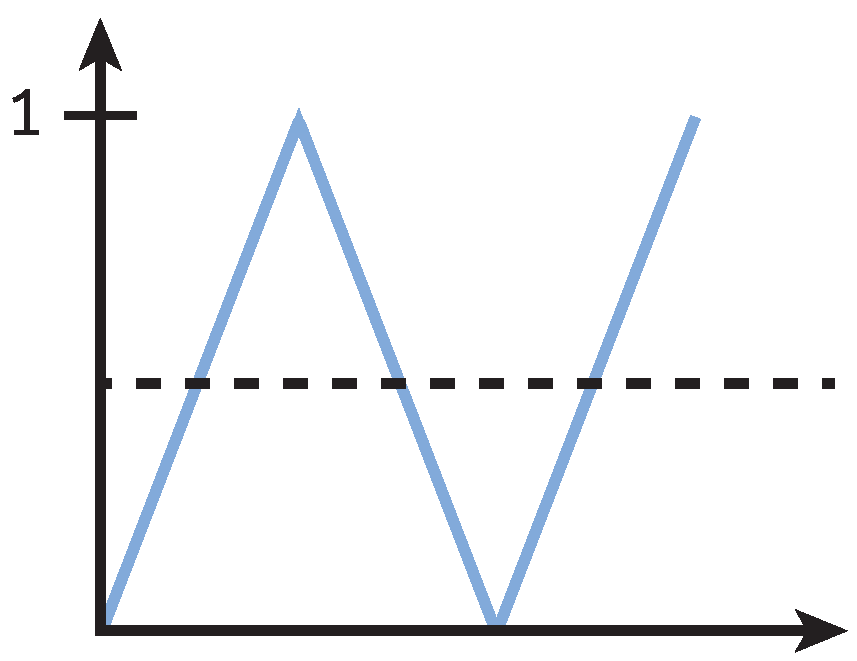
\includegraphics{FIGURES/total_variation}}
\caption[Illustration of a quantity fluctuating about a fixed point]{\label{fig:TV} Illustration of a quantity fluctuating between 0 and 1 about a fixed value.}
\end{center}
\end{figure}
We can compare the sum of the absolute value of the differences between the four points,
\begin{equation}\label{eq:sum_abs_tv}
\displaystyle \sum_{i=1}^{4}|Y(i+1)-Y(i)| = |1-0| + |0-1| + |1-0| = 3
\end{equation}
to the absolute value of the sum of the differences,
\begin{equation}\label{eq:abs_sum_tv}
|\displaystyle \sum_{i=1}^{4}(Y(i+1)-Y(i))| = |(1-0)+(0-1)+(1-0)| = 1
\end{equation}
The ratio of Eq.~(\ref{eq:sum_abs_tv}) and Eq.~(\ref{eq:abs_sum_tv}) is 3, which indicates that this data is fluctuating. For the implementation of this scheme in FDS, instead of comparing directly to 3, we use 2.9 because floating point division might not return a value of exactly 3. If fluctuations have been identified, then the values at the fourth point in the stencil are frozen and become the final values at the end of an integration time step. This prevents unnecessary sub-time steps being taken by the integrator. Because the error controller is bounding the solution, any one of the values within the stencil is also within the error tolerance and is therefore acceptable.

\chapter{The Unmixed Fraction}
\label{app:unmixed_fraction}

In Sec.~\ref{sec:subgrid_evironment} we present the evolution equation for an important variable, the unmixed fraction, $\zeta$, in the batch reactor model for turbulent combustion.  This appendix explains the development of that equation.

\subsection*{Moments of the PDF Transport Equation}
\label{app:pdf_transport}

The cell mean mass fraction of species $\alpha$ is denoted $\widetilde{Y}_\alpha(t)$. A fluid parcel at any point within the cell exists in one of two states: completely unmixed or completely mixed.  Let $\hat{Y}_\alpha(t)$ denote the mass fraction of $\alpha$ in the mixed reactor zone, initially equal to the cell mean, $\hat{Y}_\alpha(0) = \widetilde{Y}_{\alpha}^0 \equiv \widetilde{Y}_{\alpha}(0)$.  With $\psi_\alpha \in [0,1]$ representing the sample space for the composition, the subgrid probability density function (PDF) may be written as
\begin{equation}
\label{eq:pdf}
f(\psi_\alpha;t) = w_1 \delta(0-\psi_\alpha) + w_2 \delta(1-\psi_\alpha) + w_3 \delta(\hat{Y}_\alpha[t] - \psi_\alpha)
\end{equation}
where $\delta(x)$ is the Dirac delta function.  In other words, if we look at a specific point, the mass fraction of species $\alpha$ may only be 0, 1, or equal to the mixed zone value, $\hat{Y}_\alpha$ (see Fig.~\ref{fig_subgrid_environment}).  The weights $w_i$ must satisfy integral constraints on the cell: $\int f(\psi_\alpha;t) \d \psi_\alpha = 1$, $\int f(\psi_\alpha;t) \psi_\alpha \d \psi_\alpha = \widetilde{Y}_\alpha(t)$.

\begin{figure}
\begin{center}
\begin{tikzpicture}[scale=0.75]
\begin{axis}[
    width=0.95\linewidth,
    axis equal image,
    enlargelimits=false,
    axis x line=none,
    axis y line=none,
    colorbar,
    point meta min=0, point meta max=1,
    colormap={whiteblack}{gray(0cm)=(0); gray(1cm)=(1)},
    colorbar style={
        title=Mass Fraction,
        at={(1.05,0.01)}, % Coordinate system relative to the main axis. (1,1) is upper right corner of main axis.
        anchor=south west,
        height=.98*\pgfkeysvalueof{/pgfplots/parent axis height}, % Scale the colorbar relative to the main axis
        /pgf/number format/.cd, % Change the key directory to /pgf/number format
        fixed, fixed zerofill, precision=1,
        /tikz/.cd  % Change back to the normal key directory
    }
    	]
	\addplot graphics [xmin=-2.10, xmax=-0.1, ymin=-1, ymax=1] {FIGURES/transport_vs_mixing_0461_b}
	node [above,white] at (30,15) {\Large(a)};
	\addplot graphics [xmin= 0.10, xmax= 2.1, ymin=-1, ymax=1] {FIGURES/transport_vs_mixing_0461_a}
	node [above,white] at (250,15) {\Large(b)};
\end{axis}
\end{tikzpicture}
\end{center}
\caption[Idealized subgrid environment for batch reactor model]{Subgrid environment at an instant in time in a hypothetical computational cell (batch reactor). (a) Well-resolved scalar field, highly unmixed, after turbulent transport. (b) Idealized subgrid environment: the local mass fraction is either 0, 1, or equal to a mixed mean.  In the present model, the gray region is called the ``mixed reactor zone'' and evolves in time (in volume and composition) during the integration of the batch reactor.}
\label{fig_subgrid_environment}
\end{figure}

For convenience, we define the \emph{unmixed fraction}, $\zeta(t)$, as the fraction of mass within the cell existing as either 0 or 1.  To satisfy the integral constraints, the PDF weights are set to
\begin{align}
w_1 &= \zeta \, (1 - \widetilde{Y}_\alpha^0) \\
w_2 &= \zeta \, \widetilde{Y}_\alpha^0 \\
w_3 &= 1-\zeta
\end{align}
As discussed by Pope \cite{Pope:2000}, the PDF (\ref{eq:pdf}) evolves by the Fokker-Planck equation:
\begin{equation}
\label{eq:fokker-planck}
\frac{\partial f}{\partial t} = -\frac{\partial}{\partial \psi_\alpha} \left(f \left\langle \left. \frac{\partial Y_\alpha}{\partial t} \right| \psi_\alpha \right\rangle \right) \,\mbox{.}
\end{equation}
The term on the right in angled brackets is a conditional mean.  Here it is modeled using a variant of IEM \cite{Dopazo:1974} which we call {\em interaction by exchange with the mixed mean} or IEMM.  When including chemical reaction, the conditional mean is modeled by
\begin{equation}
\label{eq:iem2}
\left\langle \left. \frac{\partial Y_\alpha}{\partial t} \right| \psi_\alpha \right\rangle = \frac{1}{\tau_{\si{mix}}}(\hat{Y}_\alpha - \psi_\alpha) + \frac{\d \hat{Y}_\alpha}{\d t} \,\mbox{.}
\end{equation}
Using (\ref{eq:iem2}), the zeroth moment of (\ref{eq:fokker-planck}) yields (\ref{eq:final_comp}).  The zeroth and first moments of (\ref{eq:fokker-planck}) combine to yield the model for the chemical source term (\ref{mass_prod_rate}), once multiplied by density.

\subsection*{Derivation of First Moment Equation}

\begin{align}
\int \psi_\beta \left[ \frac{\partial f}{\partial t} = - \frac{\partial}{\partial \psi_\alpha} \left( f \left\langle \left. \frac{\partial Y_\alpha}{\partial t} \right| \psi_\alpha \right\rangle \right) \right] \d \psi_\beta
\end{align}
LHS:
\begin{align}
\int \bigg[ \frac{\partial f \psi_\beta}{\partial t} - f \underbrace{\frac{\partial \psi_\beta}{\partial t}}_{0} \bigg] \d \psi_\beta = \frac{\d \widetilde{Y}_\beta}{\d t}
\end{align}
RHS:
\begin{multline}
\int - \psi_\beta \frac{\partial}{\partial \psi_\alpha} \left( f \left\{ \frac{1}{\tau_{\si{mix}}}(\hat{Y}_\alpha - \psi_\alpha) + \frac{\d \hat{Y}_\alpha}{\d t} \right\} \right) \d \psi_\beta =\\ - \underbrace{\int \frac{\partial}{\partial \psi_\alpha}\left[ \psi_\beta f \{ \;\;\; \} \right] \d \psi_\beta}_{\mbox{0 by Pope Exercise 12.1 \cite{Pope:2000}}} + \int f \{\;\;\;\} \underbrace{\frac{\partial \psi_\beta}{\partial \psi_\alpha}}_{\delta_{\alpha \beta}} \d \psi_\beta
\end{multline}
\begin{align}
&= \frac{1}{\tau_{\si{mix}}}(\hat{Y}_\beta - \widetilde{Y}_\beta) + (1-\zeta) \frac{\d \hat{Y}_\beta}{\d t} \notag\\
&= \frac{1}{\tau_{\si{mix}}}(\hat{Y}_\beta - [\zeta \widetilde{Y}_\beta^0 + (1-\zeta)\hat{Y}_\beta]) + (1-\zeta) \frac{\d \hat{Y}_\beta}{\d t} \notag\\
&= \frac{\zeta}{\tau_{\si{mix}}}(\hat{Y}_\beta - \widetilde{Y}_\beta^0) + (1-\zeta) \frac{\d \hat{Y}_\beta}{\d t} \label{eq:first_moment}
\end{align}

\subsection*{Evolution of the Unmixed Fraction}
\label{app:evo_unmixed}

Equation (\ref{eq:zeta}) may be derived as follows.  Differentiating (\ref{eq:final_comp}) in time we get
\begin{align}
\label{eq:diff_comp}
\frac{\d \widetilde{Y}_\alpha}{\d t}
&= \widetilde{Y}_\alpha^0 \frac{\d \zeta}{\d t} + (1-\zeta) \frac{\d \hat{Y}_\alpha}{\d t} - \hat{Y}_\alpha \frac{\d \zeta}{\d t} \notag\\
&= - \frac{\d \zeta}{\d t} (\hat{Y}_\alpha-\widetilde{Y}_\alpha^0) + (1-\zeta) \frac{\d \hat{Y}_\alpha}{\d t}
\end{align}
Comparing (\ref{eq:diff_comp}) with (\ref{eq:first_moment}) we see that during the reactor step the unmixed fraction evolves by
\begin{equation}
\label{eq:zeta_ode}
\frac{\d \zeta}{\d t} = - \frac{\zeta}{\tau_{\si{mix}}} \,\mbox{.}
\end{equation}
Note that while (\ref{mass_prod_rate}) invokes (\ref{eq:zeta_ode}) in its derivation, (\ref{eq:first_moment}) does not---it is an independent derivation that relies on the choice of mixing model, in this case a variant of IEM as shown in (\ref{eq:iem2}).



\chapter{Limiting Behavior of the Turbulent Batch Reactor Model}
\label{app:eddy_dissipation_concept}
\label{source_term}

The turbulent batch reactor model, Eq.~(\ref{mass_prod_rate}), is equivalent to other approaches to modeling turbulent combustion under certain limiting conditions.  These limiting cases are discussed below.

\section{Burke-Schumann Solution}

When the reactants are initially completely mixed ($\zeta_0=0$) and the chemical kinetics are infinitely fast for a single step reaction, $\mbox{Fuel} + \mbox{Air} \rightarrow \mbox{Products}$, the present model reduces to the Burke-Schumann solution (see, e.g., \cite{Turns:1996}), where the cell mean mixture fraction is given by
\begin{equation}
\label{eq:mixture_fraction}
\widetilde{Z} = \widetilde{Y}_{\si{F}} + \left(\frac{1}{1+s}\right) \widetilde{Y}_{\si{P}} \,\mbox{.}
\end{equation}

\section{Basic EDC}

When the reactants are initially unmixed ($\zeta_0=1$) and the kinetics are infinitely fast, our model reduces to the Eddy Dissipation Concept (EDC) as described in \cite{Poinsot:TNC}.  First, write (\ref{mass_prod_rate}) for Fuel (F) with $\zeta = 1$:
\begin{equation}
\label{eq:src_zeta_1}
\dot{m}^{\prime\prime\prime}_{\si{F}} = \rho \frac{1}{\tau_{\si{mix}}} (\hat{Y}_{\si{F}} - \widetilde{Y}_{\si{F}}^0) \,\mbox{.}
\end{equation}
For infinitely fast kinetics, the Fuel composition in the mixed zone is
\begin{equation}
\label{eq:mixed_fuel_comp}
\hat{Y}_{\si{F}} = \left\{ \begin{array}{ll} 0 & \mbox{if} \quad \widetilde{Y}_{\si{F}}^0 \le \widetilde{Y}_{\si{A}}^0/s \quad \mbox{(excess Air)}  \,\mbox{,} \\
\widetilde{Y}_{\si{F}}^0 - \widetilde{Y}_{\si{A}}^0/s & \mbox{if} \quad \widetilde{Y}_{\si{F}}^0 > \widetilde{Y}_{\si{A}}^0/s \quad \mbox{(excess Fuel)}  \,\mbox{.} \end{array} \right.
\end{equation}
Using (\ref{eq:mixed_fuel_comp}) in (\ref{eq:edc}) we recover the basic EDC model:
\begin{equation}
\label{eq:edc_basic}
\dot{m}^{\prime\prime\prime}_{\si{F}} = - \rho \frac{\min(\widetilde{Y}_{\si{F}}^0,\widetilde{Y}_{\si{A}}^0/s)}{\tau_{\si{mix}}} \,\mbox{.}
\end{equation}

\section{Extended EDC}

When the unmixed fraction is held constant ($\zeta = \zeta_0$), our formulation may be cast as an extended EDC model with the mixed reactor zone treated as a perfectly stirred reactor (PSR).  Previous authors  \cite{Chen:1,Panjwani:2010,Lilleberg:2010} have referred to the mixed reactor zone as the ``fine structure region.'' In the notation of \cite{Panjwani:2010}, the extended EDC reaction rate model, comparable to (\ref{mass_prod_rate}) in this paper, is given by
\begin{equation}
\label{eq:panjwani_edc}
\rho \, \frac{\d \widetilde{Y}_\alpha}{\d t} = \rho \, \frac{\gamma_\lambda^2 \chi}{\tau^\star} \left( Y_\alpha^0 - Y_\alpha^\star \right) \,\mbox{,}
\end{equation}
where $\gamma_\lambda$ is the ``ratio between the mass of the fine structure and the total mass of the subgrid structure'' and $\chi$ is the probability of fine structure burning \cite{Panjwani:2010}; in practice, both quantities are between 0 and 1.  The reactor residence time is denoted $\tau^\star$, clearly comparable to our mixing time scale, and the fine structure mass fraction is $Y_\alpha^\star$, clearly comparable to our mixed zone mass fraction $\hat{Y}_\alpha$.  Panjwani et al.~\cite{Panjwani:2010} refer to $Y_\alpha^0$ as the mass fraction of the ``surrounding state,'' thus equivalent to our initial cell mean $\widetilde{Y}_\alpha^0$.

%\paragraph{Remarks}
%\begin{enumerate}
%\item It is not clear why $\gamma_\lambda$ should be squared in (\ref{eq:panjwani_edc}).  In fact, \cite{Chen:1} does not square this quantity.
%\item Given that $\gamma_\lambda$ and $\chi$ are in the range [0,1], the sign of the RHS of (\ref{eq:panjwani_edc}) is inconsistent since for fast chemistry $Y_{\si{F}}^\star$ may be 0 (this sign convention is used consistently by the aforementioned authors).
%\item A comparison between the models written down by \cite{Panjwani:2010} (see Eq.~(\ref{eq:panjwani_edc})) and \cite{Lilleberg:2010} makes it clear that the cell mean mass fraction may be written as $\widetilde{Y}_\alpha = (1-\gamma_\lambda^2 \chi) Y_\alpha^0 + \gamma_\lambda^2 \chi \, Y_\alpha^\star$, which is equivalent to our (\ref{eq:final_comp}) with $\zeta = 1-\gamma_\lambda^2 \chi$.  This definition of the cell mean is inconsistent with the stated definition of $\gamma_\lambda$ (quoted above) in \cite{Panjwani:2010}.
%\item Equation (\ref{eq:panjwani_edc}) may be rewritten as
%   \begin{align}
%      \label{eq:edc_compare}
%      \rho \, \frac{\d \widetilde{Y}_\alpha}{\d t} &= \rho \, \frac{(1-\zeta)}{\tau_{\si{mix}}} ( \widetilde{Y}_\alpha^0 - \hat{Y}_\alpha ) \,\mbox{,} \notag \\
%      &= \rho \, \frac{(\zeta-1)}{\tau_{\si{mix}}} ( \hat{Y}_\alpha - \widetilde{Y}_\alpha^0 ) \,\mbox{,} \notag \\
%      &= \rho \, \left[ \frac{\zeta}{\tau_{\si{mix}}}(\hat{Y}_\alpha - \widetilde{Y}_\alpha^0) + \frac{\widetilde{Y}_\alpha^0 - \hat{Y}_\alpha}{\tau_{\si{mix}}} \right] \,\mbox{.}
%   \end{align}
%   Compare (\ref{eq:edc_compare}) with (\ref{mass_prod_rate}).  Again, the first term on the RHS represents mixing, the second term reaction.  Evidently, the PSR model is
%   \begin{equation}
%      \label{eq:psr}
%      \frac{\d \hat{Y}_\alpha}{\d t} = \frac{\widetilde{Y}_\alpha^0 - \hat{Y}_\alpha}{\tau_{\si{mix}}(1-\zeta)} \,\mbox{,}
%   \end{equation}
%   where the residence time in the reactor is $\tau_{\si{mix}}(1-\zeta)$.
%\end{enumerate}

%\chapter{Derivation of the Werner Wengle Wall Model}
%%\subsubsection{R. McDermott, BFRL}
%\label{app_WWderivation}
%
%To obtain (\ref{eqn_tauwturb}) we take the first off-wall value of the streamwise velocity to be
%\begin{equation}
%\label{eqn_meanu}
%\tilde{u} = \frac{1}{\Delta z} \int_0^{\Delta z} u(z) \,\mbox{d}z \,\mbox{,}
%\end{equation}
%and then substitute the WW profile for $u(z)$ and integrate.
%
%Let $z_m$ denote the dimensional distance from wall where $z^+ = 11.81$.  Equation (\ref{eqn_meanu}) becomes
%\begin{eqnarray}
%\label{eqn_uint}
%\tilde{u} &=& \frac{1}{\Delta z} \left[ \int_0^{z_m} u(z) \,\mbox{d}z + \int_{z_m}^{\Delta z} u(z) \,\mbox{d}z \right] \,\mbox{,} \nonumber\vspace{0.2cm}\\
%&=& \frac{1}{\Delta z} \left[ \int_0^{z_m} u^+ u^* \,\mbox{d}z + \int_{z_m}^{\Delta z} u^+ u^* \,\mbox{d}z \right] \,\mbox{,} \nonumber\vspace{0.2cm}\\
%&=& \frac{1}{\Delta z} \left[ \int_0^{z_m} z^+ u^* \,\mbox{d}z + \int_{z_m}^{\Delta z} A(z^+)^B u^* \,\mbox{d}z \right] \,\mbox{,} \nonumber\vspace{0.2cm}\\
%&=& \frac{1}{\Delta z} \left[ \int_0^{z_m} \frac{z}{\ell} u^* \,\mbox{d}z + \int_{z_m}^{\Delta z} A\left(\frac{z}{\ell}\right)^B u^* \,\mbox{d}z \right] \,\mbox{,} \nonumber\vspace{0.2cm}\\
%&=& \frac{1}{\Delta z} \left[ \int_0^{z_m} \frac{z\bar{\rho}u^*}{\bar{\mu}} u^* \,\mbox{d}z + \int_{z_m}^{\Delta z} A\left(\frac{z\bar{\rho}u^*}{\bar{\mu}}\right)^B u^* \,\mbox{d}z \right] \,\mbox{,} \nonumber\vspace{0.2cm}\\
%&=& \frac{1}{\Delta z} \left[ \underbrace{\int_0^{z_m} \frac{\tau_w}{\bar{\mu}} z\,\mbox{d}z}_{I} + \underbrace{\int_{z_m}^{\Delta z} A\left(\frac{\bar{\rho}}{\bar{\mu}}\right)^B \left(\frac{\tau_w}{\bar{\rho}}\right)^{\frac{1+B}{2}} z^B\,\mbox{d}z}_{II} \right] \,\mbox{.}
%\end{eqnarray}
%
%We will integrate $I$ and $II$ separately.  First, however, we must find a way to eliminate the unknown $z_m$.  To do this we equate (\ref{eqn_wwlam}) and (\ref{eqn_wwturb}) at the point where the viscous and power law regions intersect, i.e., $z^+ = 11.81 \equiv z_m^+ = z_m \bar{\rho}u^*/\bar{\mu}$.
%\begin{eqnarray}
%\label{eqn_derivezm}
%u^+(z_m^+) = A(z_m^+)^B &=& z_m^+ \nonumber\\
%A &=& (z_m^+)^{1-B} \nonumber\\
%A^{\frac{1}{1-B}} &=& z_m^+ = \frac{z_m\bar{\rho}u^*}{\bar{\mu}} \nonumber\\
%z_m &=& \frac{\bar{\mu}A^{\frac{1}{1-B}}}{\bar{\rho}u^*} \nonumber\\
%z_m &=& \frac{(\bar{\mu}/\bar{\rho})A^{\frac{1}{1-B}}}{\sqrt{\tau_w/\bar{\rho}}} \,\mbox{.}
%\end{eqnarray}
%We now have $z_m$ in terms of $\tau_w$ and otherwise known values.
%
%Integrating section $I$ of (\ref{eqn_uint}) we find
%\begin{eqnarray}
%\label{eqn_intI}
%\int_0^{z_m} \frac{\tau_w}{\bar{\mu}} z\,\mbox{d}z &=& \frac{\tau_w}{2\bar{\mu}} \left[ z^2 \right]_0^{z_m} \nonumber\\
%&=& \frac{\tau_w}{2\bar{\mu}} z_m^2 \nonumber\\
%&=& \frac{\tau_w}{2\bar{\mu}} \frac{(\bar{\mu}/\bar{\rho})^2A^{\frac{2}{1-B}}}{\tau_w/\bar{\rho}} \nonumber\\
%&=& \frac{\bar{\mu} A^{\frac{2}{1-B}}}{2\bar{\rho}} \,\mbox{.}
%\end{eqnarray}
%
%Integrating section $II$ yields
%\begin{eqnarray}
%\label{eqn_intII}
%\int_{z_m}^{\Delta z} A\left(\frac{\bar{\rho}}{\bar{\mu}}\right)^B \left(\frac{\tau_w}{\bar{\rho}}\right)^{\frac{1+B}{2}} z^B\,\mbox{d}z &=& \left\{A\left(\frac{\bar{\rho}}{\bar{\mu}}\right)^B \left(\frac{\tau_w}{\bar{\rho}}\right)^{\frac{1+B}{2}}\right\} \frac{1}{1+B} \left[z^{1+B}\right]_{z_m}^{\Delta z} \nonumber\\
%&=& \left\{ \quad \right\} \frac{1}{1+B} \left[{\Delta z}^{1+B} - {z_m}^{1+B}\right] \nonumber\\
%&=& \left\{ \quad \right\} \frac{1}{1+B} \left[{\Delta z}^{1+B} - \left(\frac{(\bar{\mu}/\bar{\rho})A^{\frac{1}{1-B}}}{\sqrt{\tau_w/\bar{\rho}}}\right)^{1+B}\right] \nonumber\\
%&=& \left\{ \frac{A}{1+B} \left(\frac{\bar{\rho}}{\bar{\mu}}\right)^B \left(\frac{\tau_w}{\bar{\rho}}\right)^{\frac{1+B}{2}} \right\} \left[{\Delta z}^{1+B} - \frac{(\bar{\mu}/\bar{\rho})^{1+B} A^{\frac{1+B}{1-B}}}{\left(\frac{\tau_w}{\bar{\rho}}\right)^{\frac{1+B}{2}}}\right] \nonumber\\
%&=& \frac{A}{1+B} \left(\frac{\bar{\rho}}{\bar{\mu}}\right)^B \left(\frac{\tau_w}{\bar{\rho}}\right)^{\frac{1+B}{2}} {\Delta z}^{1+B} - \frac{(\bar{\mu}/\bar{\rho})}{1+B} A^{\frac{2}{1-B}} \,\mbox{.}
%\end{eqnarray}
%
%Plugging (\ref{eqn_intI}) and (\ref{eqn_intII}) back into (\ref{eqn_uint}) gives
%\begin{eqnarray}
%\label{eqn_combineint}
%\tilde{u} &=& \frac{1}{\Delta z} \left[ \frac{\bar{\mu} A^{\frac{2}{1-B}}}{2\bar{\rho}} + \frac{A}{1+B} \left(\frac{\bar{\rho}}{\bar{\mu}}\right)^B \left(\frac{\tau_w}{\bar{\rho}}\right)^{\frac{1+B}{2}} {\Delta z}^{1+B} - \frac{(\bar{\mu}/\bar{\rho})}{1+B} A^{\frac{2}{1-B}} \right] \nonumber\\
%&=& \frac{1}{2} \left(\frac{\bar{\mu}}{\bar{\rho}\Delta z}\right) A^{\frac{2}{1-B}} - \frac{1}{1+B} \left(\frac{\bar{\mu}}{\bar{\rho}\Delta z}\right) A^{\frac{2}{1-B}} + \frac{A}{1+B} \left(\frac{\bar{\rho}\Delta z}{\bar{\mu}}\right)^B \left(\frac{\tau_w}{\bar{\rho}}\right)^{\frac{1+B}{2}} \,\mbox{.}
%\end{eqnarray}
%Rearranging for $\tau_w$ we find
%\begin{eqnarray}
%\label{eqn_rearrangefortauw}
%\left(\frac{\tau_w}{\bar{\rho}}\right)^{\frac{1+B}{2}} &=& \frac{1+B}{A}\left(\frac{\bar{\mu}}{\bar{\rho}\Delta z}\right)^B \left[ \left( \frac{1}{1+B} - \frac{1}{2}\right)\left(\frac{\bar{\mu}}{\bar{\rho}\Delta z}\right)A^{\frac{2}{1-B}} + \tilde{U} \right] \nonumber\\
%&=& \frac{1-B}{2} A^{\frac{1+B}{1-B}} \left(\frac{\bar{\mu}}{\bar{\rho}\Delta z}\right)^{1+B}  + \frac{1+B}{A} \left(\frac{\bar{\mu}}{\bar{\rho}\Delta z }\right)^B \tilde{U} \nonumber\\
%\tau_w &=& \bar{\rho} \left[ \frac{1-B}{2} A^{\frac{1+B}{1-B}} \left(\frac{\bar{\mu}}{\bar{\rho}\Delta z}\right)^{1+B}  + \frac{1+B}{A} \left(\frac{\bar{\mu}}{\bar{\rho}\Delta z }\right)^B \tilde{u} \right]^{\frac{2}{1+B}} \,\mbox{,}
%\end{eqnarray}
%which corresponds to Eq. (9.46) in \cite{Sagaut:2001}.



\chapter{Scalar Boundedness Correction}
\label{app_boundedness}

Second-order central differencing of the advection term in the scalar transport equation leads to dispersion errors (spurious wiggles) and these errors, if left untreated, can lead to scalar fields which are physically not realizable, e.g., negative densities.  To prevent this, FDS employs a boundedness correction to the scalar fields after the explicit transport step.  The correction, which we describe below, acts locally and effectively adds the minimum amount of diffusion necessary to prevent boundedness violations.  This correction does not make the scalar transport scheme total variation diminishing (TVD); it only serves to correct for boundedness. Similar schemes are employed by others (e.g., \cite{Herrmann:2005}).

By default, FDS employs a TVD transport scheme (Superbee \cite{Roe:1986} for LES and CHARM \cite{Zhou:1995} for DNS). These TVD schemes are applied during the transport step and each can be shown to be TVD in one dimension under certain CFL constraints.  However, except for Godunov's scheme, the TVD proofs do not extend to three dimensions~\cite{Toro}.  Still, these schemes do a much better job than pure central differencing at mitigating dispersion error.  Note that even though TVD schemes are applied, FDS still checks for boundedness in case any small violations are not prevented by the flux limiter.

\subsubsection*{A simple case}

For simplicity we start by considering a minimum boundedness violation for density in 1-D.  That is, somewhere we have $\rho < \rho_{\min}$.  Let $\rho_i^*$ denote the resulting density from the explicit transport step for cell $i$ with volume $V_i$.  Our goal is to find a correction $\delta \rho_i$ which:
\begin{enumerate}[{(}a{)}]
\item satisfies boundedness, $\rho_i = \rho_i^* + \delta \rho_i \ge \rho_{\min}$ for all $i$
\item conserves mass, $\sum_i \delta \rho_i \, V_i = 0$
\item minimizes data variation, $\sum_i |\delta \rho_i|$ (i.e., we change the field as little as possible)
\end{enumerate}
The basic idea is to apply a linear smoothing operator, $\cal L$, to the density field in regions where boundedness violations have occurred. So, the correction may be viewed as an explicit diffusion step applied to the uncorrected field with diffusion coefficient $c$:
\begin{equation}
\rho = \rho^* + c \, {\cal L} (\rho^*)
\end{equation}
To make matters simple, let us envision for the moment that the density in cell $i$ is negative but that the densities in cells $i-1$ and $i+1$ are both safely in bounds (this actually is what happens most of the time with dispersion error).  We therefore want a correction that takes mass away from $i-1$ and $i+1$ and moves it to $i$ to make up the deficit.  We know that for cell $i$ the minimum change in mass and therefore the minimum correction that will satisfy boundedness is $\delta \rho_i = \rho_{\min} - \rho_i^*$.  The operator $\cal L$ takes the form of the standard discrete Laplacian.  The correction for cell $i$ is simply
\begin{align}
\label{eqn_rhocor}
\rho_i &= \rho_i^* + \delta \rho_i \nonumber\\
&= \rho_i^* + \rho_{\min} - \rho_i^* \nonumber\\
&=  \rho_i^* + c_i (\rho_{i-1}^* - 2 \rho_i^* + \rho_{i+1}^*)
\end{align}
Comparing the second and third lines, we find that the diffusion coefficient is given by
\begin{equation}
\label{eqn_diffcoef}
c_i = \frac{\rho_{\min} - \rho_i^*}{\rho_{i-1}^* - 2 \rho_i^* + \rho_{i+1}^*}
\end{equation}
Based on the third line of (\ref{eqn_rhocor}), the correction for cell $i$ may be thought of as the sum of the two mass fluxes from its neighboring cells.  The change in mass of cell $i$ is $\delta m_i = \delta \rho_i V_i$ and is balanced by changes in mass for cells $i-1$ and $i+1$:
\begin{align}
\delta m_{i-1} &= - c_i \, (\rho_{i-1}^* - \rho_i^*) \, V_i \notag\\
\delta m_{i+1} &= - c_i \, (\rho_{i+1}^* - \rho_i^*) \, V_i \notag
\end{align}
In this case the sum of the mass corrections is zero, as desired:
\begin{align}
\sum_{j=i-1}^{i+1} \delta m_j &= \delta \rho_{i-1} V_{i-1} + \delta \rho_i V_i + \delta \rho_{i+1}V_{i+1} \notag\\
&= - c_i \, (\rho_{i-1}^* - \rho_i^*) \, V_i + c_i \, (\rho_{i-1}^* - 2 \rho_i^* + \rho_{i+1}^*) \, V_i - c_i \, (\rho_{i+1}^* - \rho_i^*) \, V_i \notag\\
&= 0 \notag
\end{align}

\subsubsection*{Realistic cases}

The discussion above was to provide a simple case for understanding the basic idea behind the correction method.  In a realistic case we must account for multi-dimensional aspects of the problem and for the possibility that neighboring cells may both be out of bounds.  Consider a grid cell whose
density is outside the specified range. Denote this cell with a ``$c$'' for center. Its volume is $V_c$ and density is $\rho_c^*$, obtained from the transport scheme.  Let the subscript ``$n$'' denote any of the six neighboring cells (in other words, only include cells which share a face with cell $c$).  We want to correct any boundedness violations for the  cell $c$ by shifting mass to or from its neighboring cells $n$:
\begin{equation}
\rho_c = \rho_c^* + \delta \rho_c \quad ; \quad \rho_n = \rho_n^* + \delta \rho_n
\end{equation}
We first define the total amount of mass we wish to shift:
\be m_c = | \rho^*_c - \rho_{\rm cut} | \, V_c  \ee
where $\rho_{\rm cut}$ is the appropriate upper or lower bound of the density.
The amount of mass each neighboring cell can accommodate without falling outside the range is:
\be m_n = \Big| \min \Big[ \rho_{\max} , \max[\rho_{\min},\rho_n^*] \Big] - \rho_{\rm cut} \Big| \, V_n \ee
The correction terms that guarantee mass conservation ($V_c \, \delta \rho_c = - \sum V_n \, \delta \rho_n$) are:
\be
\label{eqn_rhomn}
\delta \rho_c = \pm \min \left[ m_c , \sum m_n \right] / V_c  \quad ; \quad
\delta \rho_n = \mp \min \left[ \frac{m_c}{\sum m_n} , 1 \right] m_n/V_n
\ee
Next, to correct species mass fractions that are out of bounds, we follow the exact same procedure.
\begin{equation}
Z_c = Z_c^* + \delta Z_c \quad ; \quad Z_n = Z_n^* + \delta Z_n
\end{equation}
We define the amount of species mass we wish to shift:
\be m_c = | Z^*_c - Z_{\rm cut} | \, \rho_c \, V_c  \ee
where $Z_{\rm cut}$ is either 0 or 1.
The amount of species mass each neighboring cell can accommodate without falling outside the range is:
\be m_n = \Big| \min \Big[ 1 , \max[0,Z_n^*] \Big] - Z_{\rm cut} \Big| \, \rho_n \, V_n \ee
The correction terms that guarantee mass conservation ($V_c \, \rho_c \, \delta Z_c = - \sum V_n \, \rho_n \, \delta Z_n$) are:
\be
\label{eqn_Zmn}
\delta Z_c = \pm \min \left[ m_c , \sum m_n \right] / (\rho_c \, V_c)  \quad ; \quad
\delta Z_n = \mp \min \left[ \frac{m_c}{\sum m_n} , 1 \right] m_n/(\rho_n \, V_n)
\ee


%\subsubsection{An alternate view by R. McDermott}
%
%The discussion above was to provide a simple case for understanding the basic idea behind the correction method.  In a realistic case we must account for multi-dimensional aspects of the problem and for the possibility that neighboring cells may both be out of bounds.  Here again we examine the case of a minimum density boundedness violation. Consider the cell $i$ in a 3D flow with volume $V_i$ and density $\rho_i^*$ obtained from the transport scheme.  Let ${\sf N}$ denote the set of cells containing $i$ and its neighbors, excluding diagonal neighbors (in other words, only include cells which share a face with $i$). We want to correct any boundedness violations for the $i$th cell via
%\begin{equation}
%\rho_i = \rho_i^* + \delta \rho_i
%\end{equation}
%
%To determine $\delta \rho_i$ we must consider the mass exchange between neighboring cells. Let $\delta \rho_{ji}$ denote the density change for cell $j$ in ${\sf N}$ due to a boundedness violation in $i$.  For example, if $\rho_i^* < \rho_{min}$ then the density in $i$ will increase by drawing mass from its neighbors (if the mass is available).  The mass exchange matrix is given by
%\begin{equation}
%\label{eqn_rhoij}
%\delta \rho_{ji} = \left\{ \begin{array}{ll}  \displaystyle \max(0,\rho_{min} - \rho_i^*) & \mbox{if} \quad j=i  \\ \displaystyle -c_i( \max[\rho_{min},\rho_j^*] - \max[\rho_{min},\rho_i^*]) & \mbox{if} \quad j\ne i \end{array} \right.
%\end{equation}
%The smoothing parameter in (\ref{eqn_rhoij}) is obtained from
%\begin{equation}
%\label{eqn_reali}
%c_i = \frac{\max(0,\rho_{min} - \rho_i^*)}{ \sum_{j, j\ne i} ( \max[\rho_{min},\rho_j^*] - \max[\rho_{min},\rho_i^*] )}
%\end{equation}
%
%Mass conservation is obeyed because the mass increase in cell $i$ is balanced by a mass decrease by its neighbors.  In other words, the columns of $\delta \rho_{ji}$ sum to zero.  Note, however, that the mass exchange matrix is not symmetric.  The row sum gives the final mass correction for the $i$th cell:
%\begin{equation}
%\label{eqn_sumdrho}
%\delta \rho_i = \sum_j \delta \rho_{ij}
%\end{equation}


%\chapter{The Dynamic Smagorinsky Model}
%%\subsubsection{R. McDermott}
%\label{app_dynsmag}
%
%The ``subgrid-scale'' (SGS) stress, which accounts for momentum transport by unresolved eddies, emerges from decomposition of the advection term when deriving the LES equations.  It is defined as
%\begin{equation}
%\label{eqn_tau_sgs}
%\tau_{ij}^{sgs} \equiv \bar{\rho}(\widetilde{u_i u_j} - \tilde{u}_i \tilde{u}_j) \,\mbox{.}
%\end{equation}
%The deviatoric (trace free) part of the SGS stress is modeled by gradient diffusion in analogy with the viscous stress,
%\begin{equation}
%\label{eqn_tau_sgs_deviatoric}
%\tau_{ij}^{sgs} - \frac{1}{3}\tau_{kk}^{sgs} \equiv \tau_{ij}^{sgs,dev} = -2 \mu_t \left(\tilde{S}_{ij} - \frac{1}{3}\tilde{S}_{kk}\delta_{ij}\right) =  -2 \mu_t \left(\tilde{S}_{ij} - \frac{1}{3} (\nabla\!\cdot\tilde{\mathbf{u}}) \delta_{ij}\right) \,\mbox{.}
%\end{equation}
%In FDS, the turbulent viscosity is obtained from the Smagorinsky model,
%\begin{equation}
%\label{eqn_mu_turb}
%\mu_t = \bar{\rho}(C_s \Delta)^2 |\tilde{S}| \,\mbox{,}
%\end{equation}
%where $C_s$ is the model constant and $\Delta$ is the filter width taken as the geometric average of the local mesh spacing; for example, in 3D, $\Delta = (\delta x \,\delta y \,\delta z)^{1/3}$.  Note that the quantity $(C_s \Delta)$ is the local ``mixing length'' and that $|\tilde{S}|$ provides the time scale for turbulent diffusion.
%
%In preparation for the dynamic procedure, we rewrite the model for the deviatoric SGS stress as
%\begin{equation}
%\label{eqn_tau_sgs_deviatoric2}
%\tau_{ij}^{sgs,dev} = -2 (C_s \Delta)^2 \beta_{ij} \,\mbox{,}
%\end{equation}
%defining
%\begin{equation}
%\label{eqn_beta}
%\beta_{ij} = \bar{\rho} |\tilde{S}| \left(\tilde{S}_{ij} - \frac{1}{3} \tilde{S}_{kk} \delta_{ij} \right)  \,\mbox{.}
%\end{equation}
%
%
%\subsubsection{The Dynamic Procedure}
%
%We will now discuss the dynamic procedure for determining $C_s$, the Smagorinsky constant.  The procedure itself is a series of explicit filtering operations leading to a simple algebraic relationship for $C_s(\mathbf{x},t)$ (see Eq.~(\ref{eqn_lengthscale}) below).  The FDS implementation basically follows the works of Germano et al. \cite{Germano:1991}, Moin et al. \cite{Moin:1991}, and Pino Martin et al. \cite{PinoMartin:2000}.
%
%To derive the procedure, first, we apply a ``test'' filter of width $\hat{\Delta}>\Delta$ to the LES equations to obtain
%\begin{equation}
%\label{eqn_testfiltns}
%\frac{\partial \widehat{\overline{\rho u_i}}}{\partial t} + \frac{\partial \widehat{\overline{\rho u_i u_j}}}{\partial x_j} = -\frac{\partial \widehat{\overline{\sigma}}_{ij}}{\partial x_j} \,\mbox{,}
%\end{equation}
%where $\sigma_{ij}$ is the total stress tensor. The $\,\,\breve{}\,\,$ is adopted from Pino Martin et al.~\cite{PinoMartin:2000} for the Favre test filter, $\widehat{\overline{\rho}} \breve{\widetilde{u}} \equiv \widehat{ \overline{ \rho u }}$, allowing us to rewrite Eq.~(\ref{eqn_testfiltns}) as
%\begin{eqnarray}
%\label{eqn_testfavrefiltns}
%\frac{\partial \widehat{\overline{\rho}} \breve{\widetilde{u}}_i}{\partial t} + \frac{\partial \widehat{\overline{\rho}} \breve{\widetilde{u_i u_j}}}{\partial x_j} &=& -\frac{\partial \widehat{\overline{\sigma}}_{ij}}{\partial x_j} \,\mbox{,} \nonumber\\
%\frac{\partial \widehat{\overline{\rho}} \breve{\widetilde{u}}_i}{\partial t} + \frac{\partial \widehat{\overline{\rho}} \breve{\widetilde{u}}_i \breve{\widetilde{u}}_j}{\partial x_j} &=& -\frac{\partial \widehat{\overline{\sigma}}_{ij}}{\partial x_j} - \frac{\partial T_{ij}}{\partial x_j}\,\mbox{,}
%\end{eqnarray}
%where the ``subtest'' stress is defined as
%\begin{equation}
%\label{eqn_subteststress}
%T_{ij} \equiv \widehat{\overline{\rho}} \left( \breve{\widetilde{u_i u_j}} - \breve{\widetilde{u}}_i \breve{\widetilde{u}}_j \right) \,\mbox{.}
%\end{equation}
%
%The deviatoric part of the subtest stress is modeled as,
%\begin{equation}
%\label{eqn_devtest}
%T_{ij} - \frac{1}{3}T_{kk}\delta_{ij} \equiv T_{ij}^{dev} = -2 \left( C_s \widehat{\Delta} \right)^2 \widehat{\overline{\rho}} |\breve{\widetilde{S}}|\left(\breve{\widetilde{S}}_{ij} - \frac{1}{3} \breve{\widetilde{S}}_{kk}\delta_{ij}\right)  \,\mbox{.}
%\end{equation}
%By applying the Germano identity \cite{Germano:1991}, we obtain the Leonard stress,
%\begin{eqnarray}
%L_{ij} = T_{ij} - \widehat{\tau_{ij}^{sgs}} &=& \widehat{\overline{\rho}} \left( \breve{\widetilde{u_i u_j}} - \breve{\widetilde{u}}_i \breve{\widetilde{u}}_j \right) - \widehat{ \overline{\rho} \left( \widetilde{u_i u_j} - \widetilde{u}_i \widetilde{u}_j \right)} \,\mbox{,} \nonumber\\
%&=&  \widehat{\overline{\rho}} \left( \breve{\widetilde{u_i u_j}} - \breve{\widetilde{u}}_i \breve{\widetilde{u}}_j \right) - \widehat{\overline{\rho}} \left( \breve{\widetilde{u_i u_j}} - \breve{\widetilde{u}_i \widetilde{u}_j} \right) \,\mbox{,} \nonumber \\
%\label{eqn_germano} &=&  \widehat{\overline{\rho}} \left( \breve{\widetilde{u}_i \widetilde{u}_j} - \breve{\widetilde{u}}_i \breve{\widetilde{u}}_j \right) \,\mbox{.}
%\end{eqnarray}
%Using the Favre definitions, Eq.~(\ref{eqn_germano}) may be rearranged to the form typically seen in the literature,
%\begin{eqnarray}
%L_{ij} &=&  \widehat{\overline{\rho} \frac{\overline{\rho u_i}}{\overline{\rho}} \frac{\overline{\rho u_j}}{\overline{\rho}}} - \widehat{\overline{\rho}} \frac{ \widehat{\overline{\rho u_i}}}{\widehat{\overline{\rho}}} \frac{\widehat{\overline{\rho u_j}}}{\widehat{\overline{\rho}}} \,\mbox{,} \nonumber \\
%&=& \widehat{\frac{\overline{\rho u_i}\, \overline{\rho u_j}}{\overline{\rho}}} - \frac{ \widehat{\overline{\rho u_i}} \,\widehat{\overline{\rho u_j}}}{\widehat{\overline{\rho}}} \,\mbox{,} \nonumber \\
%\label{eqn_leonard} &=& \widehat{\overline{\rho} \widetilde{u}_i \widetilde{u}}_j - \frac{ \widehat{\overline{\rho} \widetilde{u}}_i \widehat{\overline{\rho} \widetilde{u}}_j }{ \widehat{\overline{\rho}} } \,\mbox{.}
%\end{eqnarray}
%\LaTeX\,has a hard time covering the entire term with the ``wide'' version of the hat, but please note that the entire first term of Equation \ref{eqn_leonard} is test filtered. The Leonard term is computable from resolved LES values.
%
%If we now look at the \emph{model} for the Germano identity (the deviatoric part) we have,
%\begin{equation}
%\label{eqn_germanomodel}
%L_{ij}^{dev} = T_{ij}^{dev} - \widehat{\tau_{ij}^{sgs,dev}} \approx - 2\left(C_s \widehat{\Delta}\right)^2 \widehat{\overline{\rho}} |\breve{\widetilde{S}}| \left( \breve{\widetilde{S}}_{ij} - \frac{1}{3} \breve{\widetilde{S}}_{kk} \delta_{ij} \right) +  2 \left(C_s \Delta \right)^2 \widehat{\beta}_{ij} \,\mbox{.}
%\end{equation}
%Note that the entire last term should be test filtered, since $C_s$ is not necessarily uniform.  However, without pulling the length scale out of the filter operation it is difficult to compute a value for $C_s$.
%
%We now rearrange (\ref{eqn_germanomodel}) to facilitate coding,
%\begin{equation}
%\label{eqn_codemodel}
%L_{ij}^{dev} = \left(C_s \Delta\right)^2 M_{ij}^{dev} \,\mbox{,}
%\end{equation}
%where,
%\begin{equation}
%\label{eqn_Mij}
%M_{ij}^{dev} = 2\left(\widehat{\beta}_{ij} - \alpha \widehat{\overline{\rho}} |\breve{\widetilde{S}}| \left( \breve{\widetilde{S}}_{ij} - \frac{1}{3}\breve{\widetilde{S}}_{kk} \delta_{ij} \right) \right) \,\mbox{,}
%\end{equation}
%and $\alpha = (\widehat{\Delta}/\Delta)^2$.  For a test filter two times the grid width it appears we should have $\alpha = 4$.  However, as discussed by Lund \cite{Lund:1997}, the method of discrete quadrature significantly affects the results. If using the trapezoid rule, as we do in FDS, then $\alpha = 6$.
%
%We can now compute $L_{ij}$ and $M_{ij}^{dev}$ from known LES quantities.  If we right multiply Eq.~(\ref{eqn_codemodel}) by $M_{ij}^{dev}$, we obtain our desired result:
%\begin{equation}
%\label{eqn_lengthscale}
%\left(C_s \Delta\right)^2 = \frac{ L_{ij}^{dev} M_{ij}^{dev} }{ M_{ij}^{dev} M_{ij}^{dev} } \,\mbox{.}
%\end{equation}
%
%\subsubsection{Notes on implementation}
%
%\begin{enumerate}
%\item
%It is unnecessary to compute the deviatoric part of the Leonard term.  This is because, fortunately, $L_{ij} M_{ij}^{dev} = L_{ij}^{dev} M_{ij}^{dev}$.  Here's the proof (thanks to Stas Borodai of Reaction Engineering International):
%\begin{eqnarray}
%L_{ij} M_{ij}^{dev} &=& L_{ij} \left( M_{ij} - \frac{1}{3}M_{kk}\delta_{ij} \right) \,\mbox{,} \nonumber \\
%&=& L_{ij} M_{ij} - \frac{1}{3} L_{ij}\delta_{ij} M_{kk} \,\mbox{,} \nonumber \\
%\label{eqn_LMD} &=& L_{ij} M_{ij} - \frac{1}{3} L_{qq} M_{kk} \,\mbox{.}
%\end{eqnarray}
%\begin{eqnarray}
%L_{ij}^{dev} M_{ij}^{dev} &=& \left( L_{ij} - \frac{1}{3}L_{qq}\delta_{ij} \right) \left( M_{ij} - \frac{1}{3}M_{kk}\delta_{ij} \right) \,\mbox{,} \nonumber \\
%&=& L_{ij} M_{ij} - \frac{1}{3} L_{ij}\delta_{ij} M_{kk} - \frac{1}{3} M_{ij}\delta_{ij} L_{qq} + \frac{1}{9} \delta_{ij} \delta_{ij} L_{qq} M_{kk} \,\mbox{,} \nonumber \\
%&=& L_{ij} M_{ij} - \frac{1}{3} M_{kk} L_{qq} - \frac{1}{3} L_{qq} M_{kk} + \frac{1}{3} M_{kk} L_{qq} \,\mbox{,} \nonumber \\
%\label{eqn_LDMD} &=& L_{ij} M_{ij} - \frac{1}{3} L_{qq} M_{kk} \,\mbox{.}
%\end{eqnarray}
%Equations (\ref{eqn_LMD}) and (\ref{eqn_LDMD}) are equal and so there is no need to go to the trouble of subtracting the isotropic part out of $L_{ij}$.
%\item
%The length scale should be averaged over some homogeneous region to maintain stability,
%\begin{equation}
%\label{eqn_finallengthscale}
%\left(C_s \Delta\right)^2 = \frac{ \langle L_{ij} M_{ij}^{dev} \rangle}{ \langle M_{ij}^{dev} M_{ij}^{dev} \rangle } \,\mbox{.}
%\end{equation}
%In FDS, the brackets denote a spatial average over the test filter width.  If the denominator is zero, the constant is set to zero.
%\item
%It is common practice to ``clip'' the eddy viscosity.  In theory, a negative value of the eddy viscosity produces backscatter of energy from unresolved to resolved motions.  If this sounds dangerous from a stability perspective, it is.  The simple solution is to set $C_s = 0$, if $\langle L_{ij}M_{ij}^{dev} \rangle < 0$.
%\end{enumerate}


\chapter{Lilly's Analysis for Turbulent Flows}
\label{app:lilly_analysis}

The constants for the Smagorinsky and Deardorff turbulence models are not wholly empirical.  They may be derived by assuming an inertial range Kolmogorov spectrum and ``production equals dissipation''.  This analysis for Smagorinsky is attributed to D.~K.~Lilly \cite{Lilly:1967}, and may also be found in Sagaut \cite{Sagaut:2001}.  For Deardorff, this analysis is the solution to Exercise 13.45 in Pope \cite{Pope:2000}.

\subsubsection*{Smagorinsky}

The assumption that the mean production of subgrid-scale kinetic energy ($\mathcal{P}_{sgs}$) equals the mean dissipation rate ($\varepsilon$) implies (here I am being cavalier with my mean quantities)
\begin{equation}
\label{eqn_prod_eq_diss}
\mathcal{P}_{sgs} = \varepsilon
\end{equation}
Using (\ref{eqn_ke_dissipation}) at high Reynolds number ($\mu_t \gg \mu$) for an incompressible flow ($\nabla\!\cdot\mathbf{u} = 0$), (\ref{eqn_prod_eq_diss}) leads to
\begin{equation}
2\nu_t \tilde{S}_{ij}\tilde{S}_{ij} = 2\nu S_{ij} S_{ij}
\end{equation}
The components of the strain tensor $S_{ij}$ are greater in magnitude than the filtered strain components $\tilde{S}_{ij}$ and so the turbulent viscosity, $\nu_t$, must be larger than the molecular viscosity $\nu$, as would be expected.

We assume the filter width, $\Delta$, is in the inertial subrange of a high Reynolds number flow.  There the Kolmogorov kinetic energy spectrum may be written as
\begin{equation}
\label{eqn_kolmogorov}
E(k) = C_K \varepsilon^{2/3} k^{-5/3}
\end{equation}
displaying the famous ``minus five-thirds'' scaling.  The Kolmogorov constant is usually take to be $C_K \approx 1.5$.

Using the filtered dissipation spectrum (see Pope \cite{Pope:2000}), the Kolmogorov spectrum (\ref{eqn_kolmogorov}), and assuming a spectral cutoff filter we may write
\begin{align}
2 \nu \tilde{S}_{ij}\tilde{S}_{ij} &= 2 \nu \int_0^{\frac{\pi}{\Delta}} k^2 E(k) \,\d k \\
&= 2 \nu C_K \varepsilon^{2/3} \int_0^{\frac{\pi}{\Delta}} k^{1/3} \,\d k
\end{align}
Dividing by $\nu$ gives
\begin{align}
2 \tilde{S}_{ij}\tilde{S}_{ij} &= 2 C_K \varepsilon^{2/3} \frac{3}{4} \left[ k^{4/3} \right]_0^{\frac{\pi}{\Delta}} \\
|\tilde{S}|^2 &= C_K \varepsilon^{2/3} \frac{3}{2} \left(\frac{\pi}{\Delta}\right)^{4/3}
\end{align}
where $|\tilde{S}| \equiv (2 \tilde{S}_{ij}\tilde{S}_{ij})^{1/2}$.  This allows us to write the dissipation rate in terms of the filtered strain magnitude:
\begin{equation}
\label{eqn_diss_strain}
\varepsilon = \left(\frac{2}{3 C_K}\right)^{3/2} \left(\frac{\Delta}{\pi}\right)^2 |\tilde{S}|^3
\end{equation}

Now, we invoke production equals dissipation.  Below, the left-hand side is the production of SGS kinetic energy.  The right-hand side is the dissipation rate in terms of the filtered strain from (\ref{eqn_diss_strain}):
\begin{align}
\label{eqn_prod_diss_2}
2 \nu_t \tilde{S}_{ij} \tilde{S}_{ij} &= \varepsilon \\
\nu_t |\tilde{S}|^2 &= \left(\frac{2}{3 C_K}\right)^{3/2} \left(\frac{\Delta}{\pi}\right)^2 |\tilde{S}|^3
\end{align}
Inserting the constant coefficient Smagorinsky model for the turbulent viscosity, $\nu_t = (C_s \Delta)^2 |\tilde{S}|$, yields
\begin{equation}
(C_s \Delta)^2 |\tilde{S}|^3 = \left(\frac{2}{3 C_K}\right)^{3/2} \left(\frac{\Delta}{\pi}\right)^2 |\tilde{S}|^3
\end{equation}
Finally, using $C_K = 1.5$ and solving for $C_s$ gives
\begin{equation}
\label{eqn_smag_const_lilly}
C_s = \left[ \frac{2}{(3)(1.5)} \right]^{3/4} \frac{1}{\pi} = 0.17
\end{equation}

\subsubsection*{Deardorff}

The turbulent viscosity for the Deardorff form of the isotropic eddy viscosity is $\nu_t = C_\nu \Delta \, k_{sgs}^{1/2}$.  In this section, we derive the value of the constant using Lilly's analysis.  To start, we require a relationship between the dissipation rate and the subgrid kinetic energy $k_{sgs}$.  This relationship does not depend on how $k_{sgs}$ is computed---it depends on the shape of the energy spectrum and on where the filter width cutoff falls in relation to that spectrum.  Here we assume a Kolmogorov spectrum at high Re with the filter width falling inside the inertial subrange.  Then the subgrid kinetic energy is well approximated by integrating the spectrum from the cutoff wave number to infinity:
\begin{align}
k_{sgs} &= \int_{\frac{\pi}{\Delta}}^\infty E(k) \,\d k \\
&= C_K \varepsilon^{2/3} \int_{\frac{\pi}{\Delta}}^\infty k^{-5/3} \,\d k \\
%&= C_K \varepsilon^{2/3} \left(\frac{-3}{2}\right) \left[ k^{-2/3} \right]_{\frac{\pi}{\Delta}}^\infty \\
%&= 0 - C_K \varepsilon^{2/3} \left(\frac{-3}{2}\right) \left(\frac{\pi}{\Delta}\right)^{-2/3} \\
&= \frac{3}{2} C_K \varepsilon^{2/3} \left(\frac{\Delta}{\pi}\right)^{2/3}
\end{align}
which rearranges to
\begin{equation}
\label{eqn_diss_ksgs}
\varepsilon = \left(\frac{2}{3 C_K}\right)^{3/2} \frac{\pi}{\Delta} \,k_{sgs}^{3/2}
\end{equation}
Equating the relationships for the dissipation rates from Smagorinsky (\ref{eqn_diss_strain}) and Deardorff (\ref{eqn_diss_ksgs}) gives
\begin{align}
\left(\frac{\Delta}{\pi}\right)^2 |\tilde{S}|^3 &= \frac{\pi}{\Delta} \,k_{sgs}^{3/2} \\
%|\tilde{S}|^3 &= \left( \frac{\pi}{\Delta} \right)^3 \,k_{sgs}^{3/2} \\
|\tilde{S}|^2 &= \left( \frac{\pi}{\Delta} \right)^2 \,k_{sgs}
\end{align}
Now, we again invoke production equals dissipation using Deardorff as the eddy viscosity model and (\ref{eqn_diss_ksgs}) for the dissipation rate:
\begin{align}
\nu_t |\tilde{S}|^2 &= \varepsilon \\
C_\nu \Delta \,k_{sgs}^{1/2} \, \left(\frac{\pi}{\Delta}\right)^2 k_{sgs} &= \left(\frac{2}{3 C_K}\right)^{3/2} \frac{\pi}{\Delta} \,k_{sgs}^{3/2}
\end{align}
Using $C_K = 1.5$ and solving for $C_\nu$ yields
\begin{equation}
C_\nu = \left[\frac{2}{(3)(1.5)}\right]^{3/2} \frac{1}{\pi} = 0.094
\end{equation}
FDS uses a value of $C_\nu = 0.1$ for the Deardorff model constant.


\chapter{Fluid-Particle Momentum Transfer}
\label{particle_momentum_transfer}

The trajectories of Lagrangian particles in FDS could be calculated with Forward Euler (FE) time integration. However, Forward Euler extracts momentum from the cell corresponding to each particle's initial position and this may cause large changes in the flow field and ultimately instability unless the time step is extremely small. Consequently, a stable, single-step approximate solution is developed and is implemented in FDS.

Several effects are neglected in this formulation. One is the effect of the change in droplet mass between  time steps. The droplet's evaporation is not coupled to this model. This is justified because the change in droplet mass per time step is small. A second neglected effect is the change in drag coefficient between time steps. This is justified because of the large uncertainties in the drag coefficients. Modeling the time derivative of the drag coefficient would not improve accuracy beyond these uncertainties, but it would slow down the computation.

\subsubsection*{Relative velocities}
Let $m_{\rm p}$ denote the particle mass, $\mathbf{u}$ the particle velocity, $A_\text{p,c}$ the particle cross-sectional area, $C_\text{d}$ the particle drag coefficient, $\rho$ the fluid mass density, $\mathbf{U}$ the fluid velocity around the particle, $V_\text{g}$ the volume occupied by the fluid in a cell, $M \equiv \rho V_\text{g}$ the fluid mass of a cell, $n_\text{p}$ the number of particles in a cell, $M_\text{p} \equiv M/n_\text{p}$ the average fluid mass per particle in a cell, and $\mathbf{g}$ the gravitational acceleration vector.

The equations of motion of the particles and fluid are formulated as follows from Newton's second law,
\begin{align}
    \label{particle_eom}
    m_{\rm p} \frac{\d \mathbf{u}}{\d t} &= - \frac{1}{2} \rho C_\text{d} A_\text{p,c} (\mathbf{u} - \mathbf{U}) |\mathbf{u} - \mathbf{U}| + m_{\rm p} \mathbf{g} \\[.1in]
    \label{fluid_eom}
    M_{\rm p} \frac{\d \mathbf{U}}{\d t} &= \frac{1}{2} \rho C_\text{d} A_\text{p,c} (\mathbf{u} - \mathbf{U}) |\mathbf{u} - \mathbf{U}|
\end{align}
The fluid Eq.\ (\ref{fluid_eom}) is a greatly simplified version of Eq.\ (\ref{momeq}). It exists to get a reasonable estimate of the momentum coupling between the fluid and particle phases. Because it neglects terms corresponding to the pressure gradient, viscosity, etc., it is at best first-order accurate when those effects exist. However, unlike first-order accurate Forward Euler, this approach is stable. Additional terms could be added to improve accuracy in certain verification test cases, however, the current approach would solve these with a Forward Euler like step, which can cause instabilities if these terms are not constant. Thus, for the moment these terms are neglected despite their potential utility.

If we define $\mathbf{u}_\text{r} \equiv \mathbf{u} - \mathbf{U}$ as the relative velocity between the fluid and the particle, we can find a single equation for the relative velocity by dividing both equations by their respective masses (i.e., $m_{\rm p}$ and $M_{\rm p}$) and then subtracting the second from the first. This result is
\begin{align}
    \frac{\d \mathbf{u}_\text{r}}{\d t} = -\frac{1}{2} \rho C_\text{d} A_\text{p,c} \left(\frac{1}{m_{\rm p}} + \frac{1}{M_{\rm p}} \right) \mathbf{u}_\text{r} |\mathbf{u}_\text{r}| + \mathbf{g} \,.
\end{align}
This equation can be written in compact form as follows:
\begin{align}
    \frac{\d \mathbf{u}_\text{r}}{\d t} = -K_{\rm p} \mathbf{u}_\text{r} |\mathbf{u}_\text{r}| + \mathbf{g} \quad ; \quad K_{\rm p} \equiv \frac{1}{2} \rho C_\text{d} A_\text{p,c} \left(\frac{1}{m_{\rm p}} + \frac{1}{M_{\rm p}} \right) \,.
\end{align}
This is the drag equation, which has no solution in terms of elementary functions. Our solution approach first finds a solution neglecting gravity and then adds in a series for the gravity terms. $\mathbf{u}_\text{r} \equiv \mathbf{u}_\text{d} + \mathbf{u}_\text{g}$ is the decomposition of $\mathbf{u}_\text{r}$. The velocities $\mathbf{u}_\text{r}$ and $\mathbf{u}_\text{d}$ both have the same initial condition, $\mathbf{u}_\text{d}(0) = \mathbf{u}_\text{r}(0) \equiv \mathbf{u}(0) - \mathbf{U}(0)$. And $\mathbf{u}_\text{d}$ satisfies the drag equation without gravity, specifically
\begin{align}
    \frac{\d \mathbf{u}_\text{d}}{\d t} = -K_{\rm p} \mathbf{u}_\text{d} |\mathbf{u}_\text{d}|
\end{align}
The solution subject to these initial conditions is
\begin{align}
    \label{ud_exact}
    \mathbf{u}_\text{d}(t) = \frac{\mathbf{u}(0) - \mathbf{U}(0)}{1 + \beta_{\rm p} t} \quad ; \quad \beta_{\rm p} \equiv K_{\rm p} |\mathbf{u}_{\text{r}}(0)|
\end{align}
We can decompose $\mathbf{u}_\text{r}$ to find a series solution for $\mathbf{u}_\text{g}$. The function $\mathbf{u}_\text{g}$ can be written $\mathbf{u_g} = \mathbf{u}_\text{r} - \mathbf{u}_\text{d}$.  So the differential equation for $\mathbf{u}_\text{g}$ is
\begin{align}
    \frac{\d \mathbf{u}_\text{g}}{\d t} = -K_{\rm p} (\mathbf{u}_\text{r} |\mathbf{u}_\text{r}| - \mathbf{u}_\text{d} |\mathbf{u}_\text{d}|) + \mathbf{g} \quad ; \quad \mathbf{u}_\text{g}(0) = \mathbf{u}_\text{r}(0) - \mathbf{u}_\text{d}(0) = 0
\end{align}
The Taylor series for $\mathbf{u}_\text{g}$ about $t = 0$ is
\begin{align}
    \mathbf{u}_\text{g}(t) = \mathbf{u}_\text{g}(0) + t \frac{\d \mathbf{u}_\text{g}}{\d t}(0) + \frac{t^2}{2} \frac{\d^2 \mathbf{u}_\text{g}}{\d t^2}(0) + \frac{t^3}{6} \frac{\d^3 \mathbf{u}_\text{g}}{\d t^3}(0) + \cdots \,.
\end{align}
The task now is to find the derivatives of $\mathbf{u}_\text{g}$ at $t = 0$. The first derivative, $\d \mathbf{u}_\text{g} / \d t(0)$, can be seen to be $\mathbf{g}$ by inspection, as we would expect from the solution without drag. The second derivative is more complicated, and we find that
\begin{align*}
    \frac{\d^2 \mathbf{u}_\text{g}}{\d^2 t} = -K_{\rm p} \frac{\d}{\d t}(\mathbf{u}_\text{r} |\mathbf{u}_\text{r}| - \mathbf{u}_\text{d} |\mathbf{u}_\text{d}|) + \frac{\d \mathbf{g}}{\d t} = -K_{\rm p} \left(|\mathbf{u}_\text{r}| \frac{\d \mathbf{u}_\text{r}}{\d t} + \mathbf{u}_\text{r} \frac{\d |\mathbf{u}_\text{r}|}{\d t} - |\mathbf{u}_\text{d}| \frac{\d \mathbf{u}_\text{d}}{\d t} - \mathbf{u}_\text{d} \frac{\d |\mathbf{u}_\text{d}|}{\d t}\right)
\end{align*}
\begin{align}
    \frac{\d^2 \mathbf{u}_\text{g}}{\d^2 t}(0) = -K_{\rm p} \left(|\mathbf{u}_\text{r}(0)| \frac{\d \mathbf{u}_\text{r}}{\d t}(0) + \mathbf{u}_\text{r}(0) \frac{\d |\mathbf{u}_\text{r}|}{\d t}(0) - |\mathbf{u}_\text{d}(0)| \frac{\d \mathbf{u}_\text{d}}{\d t}(0) - \mathbf{u}_\text{d}(0) \frac{\d |\mathbf{u}_\text{d}|}{\d t}(0)\right)
\end{align}
where
\begin{align*}
    \frac{\d \mathbf{u}_\text{r}}{\d t}(0) &= -K_{\rm p} \mathbf{u}_{\text{r}}(0) |\mathbf{u}_{\text{r}}(0)| + \mathbf{g}  \\[.1in]
    \frac{\d \mathbf{u}_\text{d}}{\d t}(0) &= -K_{\rm p} \mathbf{u}_{\text{r}}(0) |\mathbf{u}_{\text{r}}(0)|
\end{align*}
% = -K_{\rm p} \left(\frac{\d \mathbf{u} |\mathbf{u}|}{\d t} - \frac{\d \mathbf{u}_\text{d} |\mathbf{u}_\text{d}|}{\d t} \right)
The derivative of the length of the velocity vectors (speed) must now be found. It can be shown that for an arbitrary vector $\mathbf{a}$,
\begin{align*}
    \frac{\d |\mathbf{a}|}{\d t} = \left(\frac{\mathbf{a}}{|\mathbf{a}|}\right) \cdot \frac{\d \mathbf{a}}{\d t}
\end{align*}
The derivatives of the vector lengths can be written as
\begin{align}
    \frac{\d |\mathbf{u}_\text{r}|}{\d t} &= \left(\frac{\mathbf{u}_\text{r}}{|\mathbf{u}_\text{r}|}\right) \cdot \frac{\d \mathbf{u}_\text{r}}{\d t} = \left(\frac{\mathbf{u}_{\text{r}}(0)}{|\mathbf{u}_{\text{r}}(0)|}\right) \cdot (-K_{\rm p} \mathbf{u}_{\text{r}}(0) |\mathbf{u}_{\text{r}}(0)| + \mathbf{g})  \\[.1in]
    \frac{\d |\mathbf{u}_\text{d}|}{\d t} &= \left(\frac{\mathbf{u}_\text{d}}{|\mathbf{u}_\text{d}|}\right) \cdot \frac{\d \mathbf{u}_\text{d}}{\d t} = \left(\frac{\mathbf{u}_{\text{r}}(0)}{|\mathbf{u}_{\text{r}}(0)|}\right) \cdot (-K_{\rm p} \mathbf{u}_{\text{r}}(0) |\mathbf{u}_{\text{r}}(0)|)
\end{align}
Once all of this is written out and expanded, the second derivative of $\mathbf{u}_\text{g}$ at $t = 0$ is
\begin{align}
    \frac{\d^2 \mathbf{u}_\text{g}}{\d^2 t}(0) = -K_{\rm p} \left[\mathbf{u}_{\text{r}}(0) \left(\frac{\mathbf{u}_{\text{r}}(0) \cdot \mathbf{g}}{|\mathbf{u}_{\text{r}}(0)|}\right) + \mathbf{g} |\mathbf{u}_{\text{r}}(0)|\right] = - \beta_{\rm p} \left[\mathbf{u}_{\text{r}}(0) \left(\frac{\mathbf{u}_{\text{r}}(0) \cdot \mathbf{g}}{|\mathbf{u}_{\text{r}}(0)|^2}\right) + \mathbf{g}\right]
\end{align}
This has a term parallel to the initial relative velocity and a term parallel to the gravitational acceleration vector.

Assembling all these terms, $\mathbf{u}_\text{g}$ can be found to be
\begin{align}
    \label{ug_second_order}
    \mathbf{u}_\text{g}(t) = \mathbf{g} t - \frac{\beta_{\rm p} t^2}{2} \left[\mathbf{u}_{\text{r}}(0) \left(\frac{\mathbf{u}_{\text{r}}(0) \cdot \mathbf{g}}{|\mathbf{u}_{\text{r}}(0)|^2}\right) + \mathbf{g}\right] + \mathit{O}(t^3)
\end{align}
Assembling Eqs. (\ref{ud_exact}) and (\ref{ug_second_order}), the solution for $\mathbf{u}_\text{r}$ is
\begin{align}
    \label{ur_short}
    \mathbf{u}_\text{r}(t) &= \frac{\mathbf{u}_{\text{r}}(0)}{1 + \beta_{\rm p} t} + \mathbf{g} t - \frac{\beta_{\rm p} t^2}{2} \left[\mathbf{u}_{\text{r}}(0) \left(\frac{\mathbf{u}_{\text{r}}(0) \cdot \mathbf{g}}{|\mathbf{u}_{\text{r}}(0)|^2}\right) + \mathbf{g}\right] + \mathit{O}(t^3) \quad ; \quad \beta_{\rm p} \equiv K_{\rm p} |\mathbf{u}_{\text{r}}(0)| %\\
    %\label{ur_expanded}
    %\mathbf{u} - \mathbf{U} &= \frac{\mathbf{u}(0) - \mathbf{U}(0)}{1 + \beta_{\rm p} t} + \mathbf{g} t - \frac{\beta_{\rm p} t^2}{2} \left[(\mathbf{u}(0) - \mathbf{U}(0)) \left(\frac{(\mathbf{u}(0) - \mathbf{U}(0)) \cdot \mathbf{g}}{|\mathbf{u}(0) - \mathbf{U}(0)|^2}\right) + \mathbf{g}\right] + \mathit{O}(t^3) \quad ; \quad \beta_{\rm p} \equiv K_{\rm p} |\mathbf{u}(0) - \mathbf{U}(0)|
\end{align}

\subsubsection*{Particle velocities and positions}

The results of the previous section are not directly useful unless $\mathbf{U}(t)$ is known. $\mathbf{U}(t)$ can be found via the conservation of momentum and this leads to a solution for the particle velocities and positions. The fluid and particles can gain or lose momentum due to gravity. Drag forces exchange momentum between the fluid and particle, which does not change the total momentum of the system. Summing the equations of motion and integrating in time to find the total momentum at an instant, we find that
\begin{align}
    m_{\rm p} \mathbf{u}(t) + M_{\rm p} \mathbf{U}(t) &= m_{\rm p} \mathbf{u}(0) + M_{\rm p} \mathbf{U}(0) + m_{\rm p} \mathbf{g} t  \\[.1in]
    \label{part_mom_cons}
    \mathbf{u}(t) + \alpha_{\rm p} \mathbf{U}(t) &= \mathbf{u}(0) + \alpha_{\rm p} \mathbf{U}(0) + \mathbf{g} t \quad ; \quad \alpha_{\rm p} \equiv \frac{M_{\rm p}}{m_{\rm p}}
\end{align}
After recognizing that $\mathbf{u} = \mathbf{U} + \mathbf{u}_\text{r}$ and $\mathbf{u}_\text{r} \equiv \mathbf{u}_\text{d} + \mathbf{u}_\text{g}$, we can write that $\mathbf{u} = \mathbf{U} + \mathbf{u}_\text{d} + \mathbf{u}_\text{g}$ Substituting that result in and solving for $\mathbf{U}$ leads to
\begin{align*}
    \mathbf{U}(t) + \mathbf{u}_\text{d}(t) + \mathbf{u}_\text{g}(t) + \alpha_{\rm p} \mathbf{U}(t) &= \mathbf{u}(0) + \alpha_{\rm p} \mathbf{U}(0) + \mathbf{g} t  \\[.1in]
    \mathbf{U}(t) + \frac{\mathbf{u}_{\text{r}}(0)}{1 + \beta_{\rm p} t} + \mathbf{u}_\text{g}(t) + \alpha_{\rm p} \mathbf{U}(t) &= \mathbf{u}(0) + \alpha_{\rm p} \mathbf{U}(0) + \mathbf{g} t
\end{align*}
\begin{align}
    \label{mom_U_p}
    \mathbf{U}(t) = \frac{\mathbf{u}(0) + \alpha_{\rm p} \mathbf{U}(0) + \mathbf{g} t - \mathbf{u}_\text{g}}{1 + \alpha_{\rm p}} - \frac{\mathbf{u}_{\text{r}}(0)}{(1 + \beta_{\rm p} t)(1 + \alpha_{\rm p})}
\end{align}
Eq.\ (\ref{mom_U_p}) can be substituted into Eq.\ (\ref{ur_short}) to get the solution for $\mathbf{u}$.
\begin{align}
    \mathbf{u}(t) &= \mathbf{U}(t) + \frac{\mathbf{u}(0) - \mathbf{U}(0)}{1 + \beta_{\rm p} t} + \mathbf{u}_\text{g} \nonumber \\[.1in]
    &= \frac{\mathbf{u}(0) + \alpha_{\rm p} \mathbf{U}(0) + \mathbf{g} t - \mathbf{u}_\text{g}}{1 + \alpha_{\rm p}} - \frac{\mathbf{u}(0) - \mathbf{U}(0)}{(1 + \beta_{\rm p} t)(1 + \alpha_{\rm p})} + \frac{\mathbf{u}(0) - \mathbf{U}(0)}{1 + \beta_{\rm p} t} + \mathbf{u}_\text{g} \nonumber \\[.1in]
    &= \frac{\mathbf{u}(0)}{1 + \beta_{\rm p} t} + \frac{(\mathbf{u}(0) + \alpha_{\rm p} \mathbf{U}(0))\beta_{\rm p} t}{(1 + \beta_{\rm p} t)(1 + \alpha_{\rm p})} + \frac{\mathbf{g} t + \alpha_{\rm p} \mathbf{u}_\text{g}}{1 + \alpha_{\rm p}} \nonumber \\[.1in]
    &= \frac{\mathbf{u}(0)}{1 + \beta_{\rm p} t} + \frac{(\mathbf{u}(0) + \alpha_{\rm p} \mathbf{U}(0))\beta_{\rm p} t}{(1 + \beta_{\rm p} t)(1 + \alpha_{\rm p})} + \mathbf{g} t - \frac{\alpha_{\rm p} \beta_{\rm p} t^2}{2 (1 + \alpha_{\rm p})} \left[\mathbf{u}_{\text{r}}(0) \left(\frac{\mathbf{u}_{\text{r}}(0) \cdot \mathbf{g}}{|\mathbf{u}_{\text{r}}(0)|^2}\right) + \mathbf{g}\right] + \mathit{O}(t^3) \label{mom_u_p_full}
\end{align}
Integrating Eq.~(\ref{mom_u_p_full}) leads to an equation for the particle positions,
\begin{eqnarray}
    \label{mom_x_p_full}
    \mathbf{x}(t) = \mathbf{x}(0) + \left(\frac{\mathbf{u}(0) + \alpha_{\rm p} \mathbf{U}(0)}{1 + \alpha_{\rm p}}\right) t &-& \frac{\alpha_{\rm p} (\mathbf{u}(0) - \mathbf{U}(0))}{\beta_{\rm p} (1 + \alpha_{\rm p})} \text{ln}(\beta_{\rm p} t + 1) \nonumber \\[.1in]
    &+& \frac{\mathbf{g} t^2}{2} - \frac{\alpha_{\rm p} \beta_{\rm p} t^3}{6 (1 + \alpha_{\rm p})} \left[\mathbf{u}_{\text{r}}(0) \left(\frac{\mathbf{u}_{\text{r}}(0) \cdot \mathbf{g}}{|\mathbf{u}_{\text{r}}(0)|^2}\right) + \mathbf{g}\right] + \mathit{O}(t^4)
\end{eqnarray}

\subsubsection*{Implementation in FDS}

The following solutions are used to advance the particle positions forward in time by $\Delta t$ much like a normal finite-difference scheme. The exact solution is used for the case without drag.
\begin{align}
    \mathbf{u}^{n+1} &= \frac{\mathbf{u}^n}{1 + \beta_{\rm p} \Delta t} + \frac{(\mathbf{u}^n + \alpha_{\rm p} \mathbf{U}^n)\beta_{\rm p} \Delta t}{(1 + \beta_{\rm p} \Delta t)(1 + \alpha_{\rm p})} + \mathbf{g} \Delta t - \frac{\alpha_{\rm p} \beta_{\rm p} (\Delta t)^2}{2 (1 + \alpha_{\rm p})} \left[\mathbf{u}_\text{r}^n \left(\frac{\mathbf{u}_\text{r}^n \cdot \mathbf{g}}{|\mathbf{u}_\text{r}^n|^2}\right) + \mathbf{g}\right] \\[.1in]
    \mathbf{x}^{n+1} &= \mathbf{x}^n + \left(\frac{\mathbf{u}^n + \alpha_{\rm p} \mathbf{U}^n}{1 + \alpha_{\rm p}}\right) \Delta t + \frac{\alpha_{\rm p} (\mathbf{u}^n - \mathbf{U}^n)}{\beta_{\rm p} (1 + \alpha_{\rm p})} \text{ln}(\beta_{\rm p} \Delta t + 1) + \frac{\mathbf{g} (\Delta t)^2}{2} \\[.1in]
    \alpha_{\rm p} &\equiv \frac{\rho V_{\rm g}}{m_{\rm p} n_{\rm p}} \\[.1in]
    \beta_{\rm p} &\equiv \frac{1}{2} \rho C_\text{d} A_\text{p} \left(\frac{1}{m_{\rm p}} + \frac{1}{M_{\rm p}} \right) |\mathbf{u}_{\text{r}}(0)|
\end{align}
At first glance, the theoretical accuracy of the original equation for $\mathbf{x}^{n+1}$, Eq.~(\ref{mom_x_p_full}), appears to be $\mathit{O}(\Delta t^3)$. But computation reveals it is actually $\mathit{O}(\Delta t^2)$. This is due to the velocity error reducing the overall accuracy of the position solution. The $(\Delta t)^3$ term, therefore, may be dropped from Eq.~(\ref{mom_x_p_full}) without loss of accuracy.






\chapter{Simplifications of the Radiation Transport Equation}
\label{radiation_derivations}

\subsubsection*{Antti Paajanen, VTT, Finland}


The Radiation Transport Equation (RTE) for particles is given by Eq.~(\ref{RTEspray}) and repeated here:
\begin{equation}
\mathbf{s} \cdot \nabla I_{\lambda}(\mathbf{x},\mathbf{s}) = -\Big[ \kappa_{\rm p}(\mathbf{x},\lambda) + \sigma_{\rm p}(\mathbf{x},\lambda) \Big]
I_{\lambda}(\mathbf{x},\mathbf{s}) +\kappa_{\rm p}(\mathbf{x},\lambda) \; I_{{\rm b,p}}(\mathbf{x},\lambda) +
\frac{\sigma_{\rm p}(\mathbf{x},\lambda)}{4\pi}
\int_{4\pi}\Phi(\mathbf{s},\mathbf{s}') \, I_{\lambda}(\mathbf{x},\mathbf{s}') \, \rm d\mathbf{s}' \label{RTEspray2}
\end{equation}
An accurate computation of the in-scattering integral on the right hand side of Eq.~(\ref{RTEspray2}) would be extremely time consuming and require a prohibitive amount of memory because the individual intensities in each location would have to be stored. The in-scattering integral can be approximated by dividing the total $4\pi$ solid angle into a ``forward angle,'' $\delta\Omega^l$, and an ``ambient angle,'' $\delta\Omega^*=4\pi - \delta\Omega^l$.  For compatibility with the FVM solver, $\delta\Omega^l$ is set equal to the control angle given by the angular discretization.  However, it is assumed to be symmetric around the center of the control angle.  Within $\delta\Omega^l$ the intensity is $I_{\la}(\bx,\bs)$ and elsewhere it is approximated as
\be
\label{Ustar}
U^*(\bx,\la) = \frac{U(\bx,\la) - \delta\Omega^l \, I_{\la}(\bx,\bs)}{\delta\Omega^*}
\ee
where $U(\bx)$ is the total intensity integrated over the unit sphere. The in-scattering integral in Eq.~(\ref{RTEspray2}) can now be approximated as
\begin{align}
\notag \frac{\sigma_{\rm p}(\bx,\la)}{4\pi}\int_{4\pi}\Phi(\bs,\bs') \; I_{\la}(\bx,\bs')
  \; \d\bs'
  &\approx
\sigma_{\rm p}(\bx,\la) \, \left( \chi_{\rm f} \, I_{\la}(\bx,\bs) + \frac{1}{\delta\Omega^{*}} \left(1-\chi_{\rm f}\right)
\int_{\delta\Omega^{*}} I_{\la}(\bx,\bs') \; \d \bs' \right)\\[0.1in]
  &=
\sigma_{\rm p}(\bx,\la) \, \Big( \chi_{\rm f} \; I_{\la}(\bx,\bs) +
(1-\chi_{\rm f}) \, U^*(\bx,\la) \Big)
\label{SprayRTE_RHS}
\end{align}
where $\chi_{\rm f} = \chi_{\rm f}(r,\la)=\chi_{\rm f}(\bx,\la)$ is a fraction of the total intensity originally within the solid angle $\delta\Omega^l$ that is scattered
into the same angle, $\delta\Omega^l$. The calculation of $\chi_{\rm f}$ is discussed in section~\ref{forward_fraction}. Using the definition of $U^*$ in Eq.~(\ref{Ustar}), the RTE is now:
\begin{equation}
\mathbf{s} \cdot \nabla I_{\lambda}(\mathbf{x},\mathbf{s}) = -\kappa_{\rm p}(\mathbf{x},\lambda) \,
I_{\lambda}(\mathbf{x},\mathbf{s}) + \kappa_{\rm p}(\mathbf{x},\lambda) \, I_{{\rm b,p}}(\mathbf{x},\lambda) +
\sigma_{\rm p}(\mathbf{x},\lambda) \left( 1-\chi_{\rm f} \right) \left( \frac{U(\mathbf{x},\lambda) - \delta\Omega^l \, I_{\lambda}(\mathbf{x},\mathbf{s})}{\delta\Omega^*} - I_{\lambda}(\mathbf{x},\mathbf{s}) \right)
\end{equation}
An effective scattering coefficient is next defined
\be
\label{effective_sigma_d}
\overline{\sigma}_{\rm p}(\bx,\la) = \frac{4\pi}{4\pi-\delta\Omega^l} \Big(1-\chi_{\rm f}(\bx,\la)\Big) \; \sigma_{\rm p}(\bx,\la)
\ee
Using Eq.~(\ref{effective_sigma_d}) and $\delta\Omega^*=4\pi - \delta\Omega^l$, the scattering coefficient can be written as:
\begin{equation}
\sigma_{\rm p}(\mathbf{x},\lambda) = \frac{\overline{\sigma}_{\rm p}(\mathbf{x},\lambda)}{4\pi} \frac{\delta\Omega^*}{\left(1-\chi_{\rm f} \right)}
\end{equation}
Substituting this in the previous form of the RTE yields:
\begin{equation}
\mathbf{s} \cdot \nabla I_{\lambda}(\mathbf{x},\mathbf{s}) = -\kappa_{\rm p}(\mathbf{x},\lambda) \,
I_{\lambda}(\mathbf{x},\mathbf{s}) +\kappa_{\rm p}(\mathbf{x},\lambda) \; I_{{\rm b,p}}(\mathbf{x},\lambda) +
\frac{\overline{\sigma}_{\rm p}(\mathbf{x},\lambda)}{4\pi} \left( U(\mathbf{x},\lambda) - \left( \delta \Omega^l
+ \delta\Omega^* \right) I_{\lambda}(\mathbf{x},\mathbf{s}) \right)
\end{equation}
Using $\delta\Omega^l+ \delta\Omega^*=4\pi $, the RTE simplifies to:
\begin{equation}
\mathbf{s} \cdot \nabla I_{\lambda}(\mathbf{x},\mathbf{s}) = -\Big[\kappa_{\rm p}(\mathbf{x},\lambda) + \overline{\sigma}_{\rm p}(\mathbf{x},\lambda)\Big]
I_{\lambda}(\mathbf{x},\mathbf{s}) +\kappa_{\rm p}(\mathbf{x},\lambda) \; I_{{\rm b,p}}(\mathbf{x},\lambda) +
\frac{\overline{\sigma}_{\rm p}(\mathbf{x},\lambda)}{4\pi} U(\mathbf{x},\lambda)
\end{equation}




\chapter{Absorption Coefficients of Liquid Fuels}
\label{app_abscoeff}

The burning rate of liquid pool fires depends in part on the convective and radiative heat feedback from the flames to the fuel surface. For large pool fires, radiation heat transfer dominates. Studies have been conducted to determine the spectra of emitted radiation~\cite{Suo-Anttila:PCT2009} as well as to characterize radiation absorption by gases within the flame~\cite{Wakatsuki:CST2008}. Depending on the fuel, thermal radiation can be absorbed at the surface or in depth. For fuels such as wood, most of the incident radiation is absorbed within a thin layer near the surface. For semi-transparent materials such as plastics or liquid fuels, thermal radiation may penetrate deeper. The in-depth radiation absorption by semi-transparent fuels has been studied for PMMA~\cite{Stoliarov:CF2009}, polymer films~\cite{Tsilingiris:ECM2003} and liquid pool fires~\cite{Suo-Anttila:PCT2009}. Most of the research related to the in-depth radiation absorption in liquids considers the boil-over of liquid pool fires on water~\cite{Broeckmann:JLPPI1995}. The effect of in-depth radiation absorption on evaporation of fuel droplets has also received some attention~\cite{Sazhin:IJHMT2004b}. Most liquids are highly selective absorbers, absorbing intensively in some wavelength regions while being transparent in others. This results in radiation transport models that are both computationally expensive and for which experimental data is scarce. In this appendix, we attempt to characterize the absorption of radiation by liquid fuels using effective absorption coefficients similar to those used in Refs.~\cite{Madhav:IJMP1995} and \cite{Manohar:JHT1995}.

Where data on absorption coefficients of liquids exists in the open literature, such as the Coblentz Society data found on the NIST Chemistry WebBook~\cite{Coblentz:1}, it usually  only contains data for wavelengths from approximately \SI{2.5}{\micro m} upwards. A large part of the total energy in the emission spectrum of flames may easily be contained in wavelengths shorter than \SI{2.5}{\micro m}. However, absorption spectra that begin from \SI{1}{\micro m} exists for a few liquids, including toluene~(\cite{Bertie:JMS2005}, \cite{Bertie:AS1994a}), methanol~\cite{Bertie:AS1993a}, benzene~\cite{Bertie:AS1993b} and water~\cite{Bertie:AS1996}. Furthermore, Ref.~\cite{Suo-Anttila:PCT2009} includes spectrally resolved transmission spectra of ethanol, heptane, JP-8, and an ethanol-toluene blend. Complex refractive index spectra for a few diesel fuels were reported in Ref.~\cite{Sazhin:IJHMT2004b}. Different diesel fuels have slightly different absorption spectra, due to differing additives. However, the data reported in Ref.~\cite{Sazhin:IJHMT2004b} can perhaps be used to obtain an order of magnitude estimate for the absorption coefficient of diesel fuel.

Often we are not interested in resolving the spectra of the transmitted radiation; rather, we are interested in modeling the total transmitted radiation. In these cases, it is convenient to write the radiation transport equations in terms of mean absorption coefficients. This is done to avoid the time-consuming integrations over all wavelengths. For this reason, a number of mean absorption coefficients have been introduced, such as the Rosselland-mean absorption coefficient and the Planck-mean absorption coefficient. These correspond to the optically-thin approximation and the Rosselland diffusion approximation of radiation transport. The absorption coefficients of liquids are highly wavelength dependent and are even transparent in some areas. In this case, the Planck-mean absorption coefficients are too large by several orders of magnitude. It is preferable to determine an effective absorption coefficient that attempts to replicate the absorption of radiation over a certain path length over which the majority of the radiation is absorbed.

Table~\ref{tbl_abscoeff} lists effective absorption coefficients for a few selected liquids. It contains two types of absorption coefficients. One type is determined by assuming the incoming radiation is blackbody radiation at a temperature of 1450~K. The other type is based on actual flame radiation spectra. If the wavenumber range is listed, then a blackbody temperature 1450~K is assumed in calculating the transmission. If the wavenumber range is not listed, then transmission data from Ref.~\cite{Suo-Anttila:PCT2009} is used. The path length is \SI{3}{\milli m} in all cases.

The assumption of blackbody radiation is adequate for sooty flames in which radiation from soot dominates the flame radiation spectra. However, for fuels with low sooting flames, the incoming radiation spectrum differs considerably from the blackbody spectrum. This explains the large difference in listed absorption coefficients for ethanol and methanol. The ethanol absorption coefficient is based on actual emission spectra of an ethanol flame, whereas the methanol absorption coefficient is calculated based on the blackbody spectrum. The correct value for methanol is likely to be closer to that of ethanol.

\begin{table}[ht]
\caption[Effective absorption coefficients for selected liquids]{Effective absorption coefficients for selected liquids.}
\centering
\begin{tabular}{l c c}
\hline\hline
Liquid                                              & Wavenumber Range (\si{1/\cm})  & Effective Absorption Coefficient, $\kappa$    \\ \hline
JP-8 \cite{Suo-Anttila:PCT2009}                     &  -                             & 301.4                                         \\
Ethanol-Toluene blend \cite{Suo-Anttila:PCT2009}    &  -                             & 680.1                                         \\
Ethanol \cite{Suo-Anttila:PCT2009}                  &  -                             & 1534.3                                        \\
Heptane \cite{Suo-Anttila:PCT2009}                  &  -                             & 187.5                                         \\
Toluene \cite{Bertie:AS1994a}                       &  436-6500                      & 160.8                                         \\
Methanol\cite{Bertie:AS1993a}                       &  2-8000                        & 52                                            \\
Water   \cite{Bertie:AS1996}                        &  1-15000                       & 1578                                          \\
Benzene \cite{Bertie:AS1993b}                       &  11.5-6200                     & 123                                           \\ \hline
\end{tabular}
\label{tbl_abscoeff}
\end{table}




\chapter{Solving the 1-D Heat Conduction Equation}
\label{solid-phase-discretization}


The 1-D heat conduction equation in Cartesian coordinates is:
\begin{equation}
\label{heat_cond_cart}
     \rho_s c_s \frac{\partial T_s}{\partial t} = \frac{\partial}{\partial x} \left( k_s \frac{\partial T_s}{\partial x} \right) + \dot{q}'''_s
\end{equation}
In cylindrical and spherical coordinates, the equation becomes:
\begin{equation}
\label{heat_cond_cyl2}
     \rho_s c_s \frac{\partial T_s}{\partial t} = \frac{1}{r^I}\frac{\partial}{\partial r} \left( r^I k_s \frac{\partial T_s}{\partial r} \right) + \dot{q}'''_s
\end{equation}
where $I$ is 1 for cylindrical and 2 for spherical coordinates. Since for $I=0$, the Cartesian formulation is recovered, from this point on we will consider the general form of the equation~(\ref{heat_cond_cyl2}). The indexing system used for the discretization of the equations is shown in Fig.~\ref{fig_solid_nodes}. The discretization scheme is the same regardless of whether the coordinate system is Cartesian, cylindrical, or spherical. The size of the cell nearest the boundary is set by default to be
\be
\label{eq:dx1dcond}
   x_1-x_0 = \sqrt{\frac{ \dt_0 \; k_s}{\rho_s \, c_s}}
\ee
where $\dt_0$ is a somewhat arbitrary time scale set to 1. In other words, the Fourier number based on the cell size is assumed of order unity. The user has flexibility in changing both the initial cell size and the degree of stretching.


\begin{figure}[t]
\setlength{\unitlength}{.9in}
\begin{picture}(6.5,1.5)
\put(0,0){\framebox(1,1){Gas Cell}}
\put(1.00,0){\framebox(0.10,1){1}}
\put(1.10,0){\framebox(0.20,1){2}}
\put(1.30,0){\framebox(0.40,1){3}}
\put(1.70,0){\framebox(0.80,1){$T_{\rm s,4}$}}
\put(2.50,0){\framebox(1.60,1){$T_{\rm s,5}$}}
\put(4.10,0){\framebox(1.60,1){$T_{\rm s,6}$}}
\put(5.70,0){\framebox(0.80,1){$T_{\rm s,7}$}}
\put(6.50,0){\framebox(0.40,1){8}}
\put(6.90,0){\framebox(0.20,1){9}}
\put(7.10,0){\framebox(0.10,1){\parbox[c]{.1in}{1\\0}}}
\put(1.00,1){\line(-1,1){0.25}}
\put(1.10,1){\line( 0,1){0.25}}
\put(1.30,1){\line( 1,1){0.25}}
\put(7.20,1){\line( 0,1){0.25}}
\put(0.50,1.35){$x_0$}
\put(0.95,1.35){$x_1$}
\put(1.50,1.35){$x_2$}
\put(7.00,1.35){$x_{10}$}
\end{picture}
\caption[Layout of solid phase cells]{Layout of solid phase cells. In this example, each solid phase cell is stretched by a factor of 2 until the halfway point of the solid is reached, after which the cells shrink by a factor of 2. The interface between gas and solid phase is at $x_0$. The back side boundary condition is applied at $x_{10}$. ``Virtual'' cells 0 and $N+1=11$ are located to the left and right of the solid, and are the same size as cells 1 and $N=10$.}
\label{fig_solid_nodes}
\end{figure}

The temperature at the center of each solid cell, $T_{s,i}$, is updated in time using a Crank-Nicolson scheme:

\begin{align}
\label{crank-nicolson}
(\rho_s \, c_s)_i \frac{T_{s,i}^{n+1}-T_{s,i}^{n}}{\delta t}
& = \frac{1}{2 \, r_{c,i}^I \, \delta r_i} \left( r_{i}^{I} \, k_{s,i+\frac{1}{2}} \frac{T_{s,i+1}^{n}-T_{s,i}^{n}}{\delta r_{i+\frac{1}{2}}} - r_{i-1}^{I} \, k_{s,i-\frac{1}{2}} \frac{T_{s,i}^{n}-T_{s,i-1}^{n}}{\delta r_{i-\frac{1}{2}}} \right) \notag \\[0.1in]
& +\frac{1}{2 \, r_{c,i}^I \, \delta r_i} \left( r_{i}^{I} \, k_{s,i+\frac{1}{2}} \frac{T_{s,i+1}^{n+1}-T_{s,i}^{n+1}}{\delta r_{i+\frac{1}{2}}} - r_{i-1}^{I} \, k_{s,i-\frac{1}{2}} \frac{T_{s,i}^{n+1}-T_{s,i-1}^{n+1}}{\delta r_{i-\frac{1}{2}}} \right) + \dot{q}'''_{s,i}
\end{align}
$k_{i+\frac{1}{2}}$ is the thermal conductivity at the border of the cells $i$ and $i+1$, $\delta r_i$ is the width of cell $i$, and  $\delta r_{i+\frac{1}{2}}$ is the distance from the center of cell $i$ to the center of cell $i+1$. The radial coordinate, $r_{c,i}$, denotes the cell center:
\begin{equation}
r_{c,i}^I = \left\{
\begin{array}{ll} (r_i^2 - r_{i-1}^2)/(2 \, \delta r_i)            & I=1 \quad \hbox{(cylindrical)} \\ [0.1in]
                   \sqrt{ ( r_i^3 - r_{i-1}^3)/(3 \, \delta r_i) } & I=2 \quad \hbox{(spherical)}
\end{array} \right.
\end{equation}
The temperatures at the front and back surface of a Cartesian slab (or center of a cylinder or sphere) are determined from the boundary conditions. In any of the coordinate systems, the boundary condition at the front surface is
\begin{equation}
\label{bc_front}
 -k_{s,1} \frac{T_{s,1}^{n+1}-T_{s,0}^{n+1}}{\delta r_{\frac{1}{2}}}
  =  \dot{q}_{c}''+\dot{q}_{r}''
\end{equation}
Note that $T_{s,0}$ does not represent the gas temperature, but rather it is used to establish the temperature gradient at the surface. Note also that the thermal conductivity is that of the first node. The convective heat flux is
\begin{equation}
\label{conv}
  \dot{q}_c'' = h \, \left( T_g - \frac{1}{2} \left( T_{s,\frac{1}{2}}^n+T_{s,\frac{1}{2}}^{n+1} \right) \right)
\end{equation}
where $T_g$ is the gas temperature in the first grid cell abutting the surface, and $T_{s,\frac{1}{2}}$ is the surface temperature, defined as the average of $T_{s,0}$ and $T_{s,1}$.
$(T^{n+1})^4$ can be approximated using a Taylor series expansion:
\begin{equation}
\label{T_taylor}
(T^{n+1})^4 \approx (T^n)^4 + 4 \, (T^n)^3 (T^{n+1}-T^n)
\end{equation}
which leads to approximation for the radiative flux
\begin{equation}
\label{radi}
\dot{q}_r'' = \dot{q}_{r, in}'' - \epsilon \sigma \, \left( T_{s,\frac{1}{2}}^{n+1} \right)^4
  \approx \dot{q}_{r, in}'' - \epsilon \sigma \, \left( T_{s,\frac{1}{2}}^n \right)^4 - 4 \, \epsilon\sigma \, \left( T_{s,\frac{1}{2}}^n \right)^3 \, \left( T_{s,\frac{1}{2}}^{n+1}-T_{s,\frac{1}{2}}^n \right)
\end{equation}
Now the front boundary condition is
\begin{equation}
\label{bc_front_2}
  -k_{s,1} \frac{T_{s,1}^{n+1}-T_{s,0}^{n+1}}{\delta r_{\frac{1}{2}}}
  \approx h \, \left( T_g - \frac{1}{2} \left( T_{s,\frac{1}{2}}^n+T_{s,\frac{1}{2}}^{n+1} \right) \right) +
  \dot{q}_{r, in}'' - 4 \, \epsilon\sigma \, \left(T_{s,\frac{1}{2}}^n \right)^3 \, T_{s,\frac{1}{2}}^{n+1} + 3 \, \epsilon\sigma \, \left( T_{s,\frac{1}{2}}^n \right)^4
\end{equation}
The wall surface temperature is defined:
\begin{equation}
\label{T_front}
  T_{s,\frac{1}{2}} = \frac{T_{s,1}+T_{s,0}}{2}
\end{equation}
and therefore the boundary condition becomes
\begin{equation}
\label{bc_front_4}
  -k_{s,1} \frac{T_{s,1}^{n+1}-T_{s,0}^{n+1}}{\delta r_{\frac{1}{2}}} + \left( \frac{h}{2} + 4 \, \epsilon\sigma \, \left( T_{s,\frac{1}{2}}^n \right)^3 \right) \frac{T_{s,1}^{n+1}+T_{s,0}^{n+1}}{2}
  \approx h\, \left( T_g - \frac{1}{2}T_{s,\frac{1}{2}}^n \right) +
  \dot{q}_{r, in}'' + 3 \, \epsilon\sigma \, \left( T_{s,\frac{1}{2}}^n \right)^4
\end{equation}

\newpage
Rearranging terms, the temperature at node 0 becomes:
\begin{equation}
\label{T0}
  T_{s,0}^{n+1} = \underbrace{\frac{\frac{k_{s,1}}{\delta r_{\frac{1}{2}}}- \left(\frac{1}{4}h+2\epsilon \sigma \left(T_{s,\frac{1}{2}}^n\right)^3 \right)}{\frac{k_{s,1}}{\delta r_{\frac{1}{2}}} + \left(\frac{1}{4}h+2\epsilon \sigma \left( T_{s,\frac{1}{2}}^n\right)^3 \right)}}_\textct{RFACF2} T_{s,1}^{n+1} +
 \underbrace{\frac{h \left(T_g-\frac{1}{2}T_{s,\frac{1}{2}}^n\right)+\dot{q}_{r,in}''+3\epsilon \sigma \left( T_{s,\frac{1}{2}}^n\right)^4}{\frac{k_{s,1}}{\delta r_{\frac{1}{2}}}+\left(\frac{1}{4}h+2\epsilon \sigma \left( T_{s,\frac{1}{2}}^n\right)^3 \right)}}_\textct{QDXKF}
\end{equation}
Note that \textct{RFACF2} and similar names are used in the actual source code to represent these quantities.
In case of non-insulated backing in Cartesian geometry, the temperature of virtual node $N+1$ is calculated the same way.
For a Cartesian geometry with an insulated backing or for cylindrical and spherical geometries, $\epsilon$, $\dot{q}_{r,in}''$, and $h$ are set to 0.

After re-arranging the terms, Eq.~(\ref{crank-nicolson}) becomes (using the nomenclature of the source code) for each wall cell $i$:
 \begin{equation}
\label{tridiagonal_1}
  B_i \; T_{i-1}^{n+1} + D_i \; T_{i}^{n+1} + A_i \; T_{i+1}^{n+1} = C_i \quad i=1,...,N
\end{equation}
where
\begin{equation}
\label{tridiagonal_2}
\begin{split}
& A_i = -\frac{k_{i+\frac{1}{2}} \, \delta t}{2(\rho_s c_s)_i} \; \frac{1}{r_{c,i}^I \delta r_i} \; \frac{r_{i}^I}{\delta r_{i+\frac{1}{2}}}  \\
& B_i = -\frac{k_{i-\frac{1}{2}} \, \delta t}{2(\rho_s c_s)_i} \; \frac{1}{r_{c,i}^I \delta r_i} \; \frac{r_{i-1}^I}{\delta r_{i-\frac{1}{2}}}   \\
& C_i = T_{s,i}^{n}-A_i \, (T_{i+1}^n-T_i^n) + B_i \, (T_{i}^n-T_{i-1}^n) + \dt \, \dot{q}_{s,i}'''/(\rho_s c_s)_i \\
& D_i = 1-A_i-B_i
\end{split}
\end{equation}
To solve Eq.~(\ref{tridiagonal_1}), a tri-diagonal linear solver is used:
\begin{equation}
\begin{split}
& C_1 = C_1 - B_1 \cdot \textct{QDXKF} \\
& C_N = C_N - A_N \cdot \textct{QDXKB} \\
& \\
& D_1 = D_1 + B_1 \cdot \textct{RFACF2} \\
& D_N = D_N + A_N \cdot \textct{RFACB2} \\
& \\
& D_i = D_i - \frac{B_i \; A_{i-1}}{D_{i-1}} \quad i = 2, ..., N-1 \\
& C_i = C_i - \frac{B_i \; C_{i-1}}{D_{i-1}} \quad i = 2, ..., N-1\\
& \\
& C_N = \frac{C_N}{D_N} \\
& \\
& T^{n+1}_{s,N} = C_N \\
& T^{n+1}_{s,i} = \frac{C_i - A_i \; C_{i+1}}{D_i} \quad i = N-1,..., 1
\end{split}
\end{equation}
